\documentclass{article}
\usepackage{graphicx} % Required for inserting images
\usepackage{authblk} % Required for author affiliations
\usepackage{indentfirst} % Indent first paragraph of sections
\usepackage{amssymb} % For mathematical symbols
\usepackage{amsthm} % For theorem environments
\usepackage{amsmath} % For advanced math typesetting
\usepackage{hyperref}
\usepackage{enumitem}
\usepackage{pgfplots} % For plots
\usepackage{tikz} % For drawing shapes
\usetikzlibrary{arrows.meta,calc}
\pgfplotsset{compat=1.18} % Set compatibility level
\newtheorem{theorem}{Theorem}
\newtheorem{corollary}{Corollary}[theorem]
\newtheorem{lemma}[theorem]{Lemma}
\newtheorem{definition}{Definition}
\newtheorem{problem}{Problem}
\newtheorem{solution}{Solution}
\newtheorem*{example}{Example}
\newtheorem{remark}{Remark}
\newtheorem{proposition}{Proposition}
\newcommand{\Span}{\operatorname{span}}
\newenvironment{amatrix}[1]{%
  \left(\begin{array}{@{}*{#1}{c}|c@{}}
}{%
  \end{array}\right)
}
\reversemarginpar
\hypersetup{
    colorlinks=true,
}
\begin{document}
%------- Title page   -----------
\title{MATH 223: Linear Algebra}
\author{William Homier}
\affil[1]{McGill University Physics, 3600 Rue University, Montréal, QC H3A 2T8, Canada}
\date{January \(5^{th}\), 2026}
\setcounter{Maxaffil}{0}
\renewcommand\Affilfont{\itshape\small}
\maketitle

%------- Abstract -----------
\noindent\rule{\textwidth}{0.4pt}
\thispagestyle{empty}
\begin{abstract}

\end{abstract}
\noindent\rule{\textwidth}{0.4pt}
\clearpage

%------- Table of Contents -----------
\thispagestyle{empty}
{
  \hypersetup{linkcolor=black}
  \tableofcontents
}
\clearpage

%------- introduction -----------
\setcounter{page}{1}
\section{Introduction}

\section{Prerequisite knowledge}
\subsection{Notation}
\subsubsection{Sets}
Sets are a grouping of objects.
\begin{center}
    \begin{tabular}{c|p{6cm}|p{5cm}}
        Set & Meaning & Examples \\
        \hline
        $\mathbb{N}$ & The set of natural numbers & (0, 1, 2, 3, ...)\\
        $\mathbb{Z}$ & The set of integers & (..., -3, -2, -1, 0, 1, 2, 3, ...)\\
        $\mathbb{Q}$ & The set of rational numbers & \(\mathbb{Q} = {\frac{a}{b}\:|\:\forall a,b \in \mathbb{Z}\:and\:b \neq 0}\)\\
        $\mathbb{R}$ & The set of all rational and all irrational numbers & \((...,-1,0,\frac{1}{4},1,1000,...)\)\\
        $\mathbb{C}$ & The set of all complex numbers & \(\mathbb{C} = \{x + iy\:|\:x,y \in \mathbb{R}\:and\:i \subseteq \sqrt{-1}\}\).\\
    \end{tabular}
\end{center}

We have the following relationships between sets:
\[\mathbb{N} \subseteq \mathbb{Z} \subseteq \mathbb{Q} \subseteq \mathbb{R} \subseteq \mathbb{C}\]
\subsubsection{Symbols}
\begin{center}
    \begin{tabular}{c|l}
        Symbol & Meaning \\
        \hline
        $\subseteq$ & is a subset of or equal to \\
        $\subset$ & is a strict subset of \\
        $\in$ & is an element of \\
        $\forall$ & for all \\
        $\exists$ & there exists \\
        $\emptyset$ & empty set \\
        $\Rightarrow$ & implies \\
        $\Leftrightarrow$ & if and only if \\
        $\cong$ & is isomorphic to
    \end{tabular}
\end{center}\footnote{is isomorphic to = structurally the same as...}

\subsection{Familiarity with $\mathbb{R}^n$}
\begin{definition}[$\mathbb{R}^n$]
Let \(n \in \mathbb{N}\). The Cartesian product of \(n\) copies of \(\mathbb{R}\) is called \(\mathbb{R}^n\).
\[\mathbb{R}^n = \{\begin{pmatrix}x_1\\\ldots\\x_n\end{pmatrix} : x_1, \ldots, x_n \in \mathbb{R}\}\]
\end{definition}

\subsection{Polar Coordinates}
\begin{definition}[Polar coordinates]
    Instead of describing a point by \((x,y)\), we may describe it using polar coordinates \((r,\theta)\), where \(r\) is the distance to the origin and \(\theta\) is the angle with the positive \(x\)-axis.
\end{definition}
\begin{example}
    Consider the point \((x,y)\), where \(x = r \cos(\theta)\:and\:y = r \sin(\theta)\). We can define \((r,\theta)\) as follows:
    \begin{center}
        \begin{tikzpicture}[scale=1.3]
            \draw[->] (-1.4,0)--(1.4,0) node[right]{$x$};
            \draw[->] (0,-1.4)--(0,1.4) node[above]{$y$};
            \coordinate (Z) at (0.9,0.5);
            \draw[fill] (Z) circle(0.02) node[above right] {$(x,y)$};
            \draw (0,0) -- (Z) node[midway, above] {$r$};
            \draw[dashed] (Z) -- (0.9,0);
            \draw[dashed] (Z) -- (0,0.5);
            \draw (0.4,0) arc (0:29:0.4);
            \node at (0.45,0.12) {$\theta$};
        \end{tikzpicture}
    \end{center}
\end{example}

\subsection{Complex Algebra}
\subsubsection{Complex Numbers}
\begin{definition}[Complex Number]
    A complex number is of the form: \(z = x + iy\) where \(x,y \in \mathbb{R}\) and \(i\) is the imaginary unit \(i = \sqrt{-1}\).
\end{definition}
\begin{theorem}[Fundamental Theorem of Algebra]
    The FTA states that any non-constant, single-variable polynomial\footnote{Polynomial is a function such as: \(f = a_n x^n + a_{n-1}x^{n-1} + ... + a_1 x + a_0\) where \(a_i \in \mathbb{R}\) or \(\mathbb{C}\) and \(n \in \mathbb{N}\).} with complex coefficients has at least one root in \(\mathbb{C}\).
\end{theorem}
\begin{remark}
    If we have a polynomial \(f\) of degree \(n\), then it has \(n\) roots, where each root can have a multiplicity\footnote{The multiplicity of a root represents how many times the root occurs in the polynomial.}.
\end{remark}
\begin{example}
    If we have a polynomial \((x-1)^2\), it has a degree of 2 but only one root, which is 1, with a multiplicity of 2.
\end{example}
We can factorize a polynomial in the form of \(f = a_n x^n + ... + a_1 x + a_0\) into a linear factor: \(f = a(x - z_1)(x - z_2)...(x - z_n)\) where \(z_i\) are the roots of \(f\) in \(\mathbb{C}\). Therefore, the FTA implies that \(f\) has a root \(f(z) = a(z-z) = 0\).
\subsubsection{Complex Operations}
\label{subsec:CO}
We can define operations on complex numbers as follows:
\begin{itemize}
    \item Addition: \(z + z' = (x + x') + i(y + y')\), where \(x,x',y,y' \in \mathbb{R}\).
    \item Multiplication: \(zz' = (x + iy)(x' + iy') = (xx' - yy') + i(xy' + yx')\).
    \item Inverse: \(\frac{1}{z} = \frac{\overline{z}}{z\overline{z}} = \frac{x - iy}{x^2 + y^2} = \frac{x}{x^2 + y^2} + i\frac{-y}{x^2 + y^2}\)
\end{itemize}
Multiplying by a complex number \(z\) corresponds geometrically to
\[\begin{cases}\text{a rotation by some angle } \theta,\\\text{a rescaling by the factor } |z|.\end{cases}\]
\subsubsection{Complex Conjugate}
\begin{definition}[Complex Conjugate]
    A complex conjugate is a way to "flip" the imaginary part of a complex number. For example, if we have a complex number \(z = x + iy\), then the complex conjugate of \(z\) is \(\overline{z} = x - iy\).
\end{definition}
Some basic properties of complex conjugates are:
\begin{itemize}
    \item \(\overline{z} = z\)
    \item \(\overline{z + z'} = \overline{z} + \overline{z'}\)
    \item \(\overline{z \cdot z'} = \overline{z} \cdot \overline{z'}\)
\end{itemize}

\marginpar{January 09, 2026.}
\subsubsection{Geometric Interpretation of Complex Numbers}
\begin{definition}[Geometric interpretation]
    Every complex number \(z = x + iy\) can be identified with a point \((x,y)\) in the plane, called the complex plane.
\end{definition}
We define the complex plane as:
\[\mathbb{C} = \{x + iy \mid x,y \in \mathbb{R}\}.\]

\begin{center}
    \begin{tikzpicture}[scale=1]
    \draw[->] (-2,0) -- (2,0) node[right] {$\Re$};
    \draw[->] (0,-2) -- (0,2) node[above] {$\Im$};
    \coordinate (z) at (1.3,0.9);
    \draw[dashed] (z) -- (1.3,0) node[below] {$x$};
    \draw[dashed] (z) -- (0,0.9) node[left] {$y$};
    \draw[thick,->] (0,0) -- (z);
    \fill (z) circle (1pt);
    \node[above right] at (z) {$z=x+iy$};
    \node[below left] at (0,0) {$0$};
    \end{tikzpicture}
\end{center}
We can rewrite the definition of the unit circle as follows:
\[S' = \{(x,y) \in \mathbb{R}^2 : x^2 + y^2 = 1\} = \{ z \in \mathbb{C} : |z| = 1\},\]
where \(S'\) is the unit circle in the complex plane.

\subsubsection{Modulus}
\begin{definition}[Modulus]
    The modulus of a complex number \(z\) is defined by
    \[|z| = \sqrt{z\overline{z}} = \sqrt{x^2 + y^2}.\]
    Geometrically, \(|z|\) is the distance from the origin to the point \((x,y)\). Recall $r$ in polar coordinates, which is the same as \(|z|\).
\end{definition}

\subsubsection{Polar Form of Complex Numbers}
\begin{definition}[Euler's formula]
    \begin{equation}
        \label{eq:EulerFormula}
        e^{i\theta} = \cos\theta + i\sin\theta
    \end{equation}
\end{definition}
\begin{definition}[Polar and exponential form]
    If $z=x+iy$ with $r=\sqrt{x^2+y^2}$, then
    \[x=r\cos\theta, \quad y=r\sin\theta,\]
    so
    \[z=r(\cos\theta+i\sin\theta)=re^{i\theta}.\]
\end{definition}
\begin{definition}[Multiplication in polar form]
    \[z = re^{i\theta}, \quad z' = r'e^{i\theta'}, \quad zz' = rr'e^{i(\theta + \theta')}.\]
\end{definition}
\begin{example}
    \[(1 + i)^{32} = (\sqrt{2}e^{i\pi/4})^{32} = (\sqrt{2})^{32} e^{i8\pi} = 2^{16}(\cos 8\pi + i \sin 8\pi) = 2^{16}.\]
\end{example}

\subsubsection{Roots in $\mathbb{C}$}
\begin{definition}[\(n^{\text{th}}\) roots in $\mathbb{C}$]
    For any complex number $z$, an $n^{\text{th}}$ root of $z$ is a complex number $w$ such that
    \[w^n = z.\]
\end{definition}
\begin{example}
    If \(z = re^{i\theta}\), then any solution of \(w^n = z\) must satisfy
    \[w_k = r^{1/n} e^{i(\theta + 2\pi k)/n}, \quad k = 0,1,2,\dots,n-1,\]
    where the $n^{\text{th}}$ roots of $z$ are equally spaced on a circle of radius $r^{1/n}$ centered at the origin.
\end{example}
\begin{definition}[Roots of unity]
The \(n^{\text{th}}\) roots of unity are the solutions of a special case where $z = 1$.
\end{definition}
\begin{example}
    If $z = 1$, then any solution of $w^n = z$ must satisfy
    \[w_k = e^{i2\pi k/n}, \quad k = 0,1,2,\dots,n-1.\]
    Geometrically, they lie on the unit circle and are equally spaced.
\end{example}

\subsection{Basic Algebraic structures}
\subsubsection{Sets with Multiplication}
\begin{definition}[Set with multiplication]
A set $M$ is called a set with multiplication if you can multiply any two elements of $M$, and the result is still in $M$.
In other words, for any $a,b \in M$, the product $ab$ is also in $M$.
\end{definition}
\begin{example}
    An example of a set with multiplication is the set of all \(2 \times 2\) complex matrices: \(M = M_2(\mathbb{C})\). Another example is the nonzero set of all real numbers \(\mathbb{R}\) with ordinary multiplication: \(\mathbb{R}^* = \mathbb{R} \setminus \{0\}\).
\end{example}
\begin{example}
Let $M = \mathbb{R}$.  
If $a,b \in \mathbb{R}$, then $ab \in \mathbb{R}$.  
So the real numbers $\mathbb{R}$ form a set with multiplication.
\end{example}

\subsubsection{Invertibility}
\begin{definition}[Condition for Invertibility]
    Let \(A \in M\) be an \(n \times n\) matrix, and suppose that there exists an \(n \times n\) matrix \(B\) such that \(AB = I_n\) or \(BA = I_n\). Where \(I_n\) is the \(n \times n\) identity matrix\footnote{An identity matrix is a square matrix with 1s on its main diagonal and 0s everywhere else. It represents no change in linear transformations, and it's used in finding matrix inverses.}$\begin{bmatrix}1&0&0\\0&\ldots&0\\0&0&1\end{bmatrix}$. Then A is invertible, and \(B\) is called the inverse of \(A\) and is denoted by \(B = A^{-1}\).
\end{definition}
\begin{remark}
    If \(A\) is invertible, then \(A^{-1}\) exists and is unique\footnote{Unique means there is exactly one such element.}.
\end{remark}

To determine if an element \(A\) in a set with multiplication \(M\) is invertible, we can use the following examples:
\begin{example}
    Let \(M = \mathbb{Z} = \{...-2,-1,0,1,2,...\}\) and \(A = 2\). Is \(A\) invertible in \(M\)?\\
    Solution: No, because \(\frac{1}{2} \notin \mathbb{Z}\).
\end{example}
\begin{example}
    Let \(M = \mathbb{R}\) and \(A = 2\), is \(A\) invertible in \(M\)?\\
    Solution: Yes, because \(\frac{1}{2} \in \mathbb{R}\).
\end{example}
\begin{example}
    Is \(1 + i\) invertible in \(\mathbb{C}\)?\\
    Solution: Yes, using our previous definition of inverse \eqref{subsec:CO}, we get that \[\frac{1}{1 + i} = \frac{1 - i}{2} \in \mathbb{C}.\]
\end{example}
\begin{problem}[Invertibility]
    Show that if an inverse of A in \(\mathbb{M}\) exists, then it is unique.
\end{problem}
\begin{problem}[Invertibility 2]
    Let \(K\) be a field. Prove that this matrix $\begin{bmatrix}0&1\\0&0\end{bmatrix}$ \(\in M_2(K)\) is not invertible.
\end{problem}

\subsubsection{Ring}
\begin{definition}[Ring]
    \label{def:Ring}
    A ring is a set $R$ where you can add and multiply elements, and the following are true:

    \begin{enumerate}
        \item You can add any two elements and stay in $R$. There is a zero, every element has a negative, and addition is commutative\footnote{Property which focuses on changing order of addition, i.e $a + b = b + a$.} and associative\footnote{Property which focuses on changing grouping of addition, i.e $a + (b + c) = (a + b) + c$.}.
        \item You can multiply any two elements and stay in $R$. Multiplication is associative, and there is a $1$.
        \item Multiplication distributes over addition:
        \[a(b+c) = ab + ac \quad \text{and} \quad (a+b)c = ac + bc.\]
    \end{enumerate}
\end{definition}
\begin{example}
    The main example of a ring is the set of integers $\mathbb{Z}$.
\end{example}

\subsubsection{Field}
\begin{definition}[Field]
    A field is a ring \textup{\eqref{def:Ring}} in which every nonzero element has a multiplicative inverse.
\end{definition}
\begin{example}
    Let $F$ be a set with two elements $F = \{0,1\}$ with addition and multiplication defined modulo $2$. The operations are given by
    \[\begin{array}{c|cc}+ & 0 & 1 \\ \hline 0 & 0 & 1 \\ 1 & 1 & 0\end{array} \qquad \begin{array}{c|cc}\cdot & 0 & 1 \\ \hline 0 & 0 & 0 \\ 1 & 0 & 1\end{array}\]
    Then $0$ is the additive identity, $1$ is the multiplicative identity, and the only nonzero element $1$ satisfies $1^{-1}=1$. Hence every nonzero element has a multiplicative inverse, so $F$ is a field.
\end{example}
\begin{problem}[Field]
    Construct a field with 2 elements.
\end{problem}

\marginpar{January 09, 2026.}
\section{Vector Spaces}
\subsection{Abstract Vector Spaces}
A regular vector space like $\mathbb{R}^n$ has concrete vectors you can see as tuples of numbers, while an abstract vector space generalizes this idea: vectors can be anything, as long as addition and scalar multiplication satisfy the vector space axioms.
\begin{definition}[Vector space over a field]
    Let $k$ be a field. A vector space over $k$ is a set $V$ with addition and scalar multiplication such that
    \[\text{(i) } v_1+v_2\in V, \qquad\text{(ii) } \lambda v\in V, \qquad\text{(iii) } 0\in V,\]
    and satisfying the usual vector space axioms (see Appendix~\ref{subsec:VSA}).\footnote{For this course, the main properties we need to know are closure under addition and scalar multiplication, and the existence of the zero vector.}
\end{definition}

\subsection{Vectors}
\subsubsection{Vector operations}
Vector operations are defined as follows:\\
\begin{itemize}
    \item Addition: \(\begin{pmatrix}x_1\\\vdots\\x_n\end{pmatrix} + \begin{pmatrix}y_1\\\vdots\\y_n\end{pmatrix} = \begin{pmatrix}x_1 + y_1\\\vdots\\x_n + y_n\end{pmatrix}\).
    \item Scalar multiplication: \(\lambda \begin{pmatrix}x_1\\\vdots\\x_n\end{pmatrix} = \begin{pmatrix}\lambda x_1\\\vdots\\\lambda x_n\end{pmatrix}\), where $\lambda \in \mathbb{R}$.
\end{itemize}
\begin{definition}[Linear combination]
    A linear combination of vectors \(v_1, \ldots, v_n\) is a vector \(v\) of the form \(v = \lambda_1v_1 + \ldots + \lambda_nv_n\), where \(\lambda_1, \ldots, \lambda_n \in \mathbb{R}\).
\end{definition}

\subsection{Span}
\marginpar{January 12, 2026.}
\begin{definition}[Span]
    Let \(A \subset \mathbb{R}^n\). The span of \(A\), denoted \(\Span(A)\), is the set of all linear combinations of elements of \(A\). In particular, if \(A=\{v_1,\ldots,v_k\}\) (where \(k\) is the number of vectors in the set), then
    \[\Span(A) = \{\lambda_1 v_1+\cdots+\lambda_k v_k : \lambda_i \in \mathbb{R}\}.\]
\end{definition}
When working in \(\mathbb{R}^n\), the span describes all points you can reach by scaling and adding the given vectors. Depending on the vectors, the span can be a line (if the vectors are dependent), a plane, or a higher-dimensional subspace.
\begin{remark}
    If \(A=\{v\}\subset \mathbb{R}^2\) with \(v\neq 0\), then
    \[\Span(v)=\{\lambda v : \lambda \in \mathbb{R}\}.\]
    This set consists of all scalar multiples of \(v\), which form a line in the direction of \(v\). In particular, taking \(\lambda=0\) gives \(0\in\Span(v)\), so the line passes through the origin.
\end{remark}

\begin{example}
    Let \(A = \begin{pmatrix}1\\1\end{pmatrix}\). Then $\Span(A) = \left\{ t\begin{pmatrix}1\\1\end{pmatrix} \mid t \in \mathbb{R} \right\},$ which is a line in \(\mathbb{R}^2\).
\end{example}
\begin{problem}[Span]
    Let \(v_1 = \begin{pmatrix}3\\1\end{pmatrix}\), \(v_2 = \begin{pmatrix}1\\3\end{pmatrix}\). Find $\Span(v_1,v_2)$.
\end{problem}
Span is a generalization of lines in \(\mathbb{R}^2\). For example, let $v_1$ and $v_2$ be two linearly independent vectors in \(\mathbb{R}^2\).
Any vector in \(\Span(v_1,v_2)\) has the form \(\lambda_1 v_1+\lambda_2 v_2\). Geometrically, this can be illustrated as the
sum of two scaled vectors.
\begin{center}
    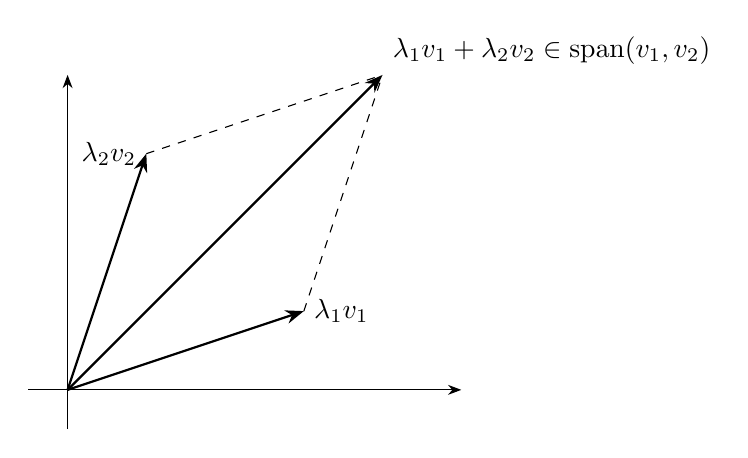
\begin{tikzpicture}[scale=1, >=Stealth]
        \draw[->] (-0.5,0) -- (5,0);
        \draw[->] (0,-0.5) -- (0,4);
        \coordinate (v1) at (3,1);
        \coordinate (v2) at (1,3);
        \draw[->, thick] (0,0) -- (v1) node[right] {$\lambda_1 v_1$};
        \draw[->, thick] (0,0) -- (v2) node[left] {$\lambda_2 v_2$};
        \draw[dashed] (v1) -- ($(v1)+(v2)$);
        \draw[dashed] (v2) -- ($(v1)+(v2)$);
        \draw[->, thick] (0,0) -- ($(v1)+(v2)$) node[above right] {$\lambda_1 v_1+\lambda_2 v_2\in \Span(v_1,v_2)$};
    \end{tikzpicture}
\end{center}
Furthermore, if \(v_1,v_2\) are linearly dependent such that $v_1 = \lambda v_2$, where $\lambda \in \mathbb{R}$ and $\lambda \neq 0$, then \(\Span(v_1,v_2)\) is a line in \(\mathbb{R}^2\) and $span(v_1) = span(v_2)$. Geometrically, this is a straight line through the origin in the direction of \(v_1\) (and \(v_2\)).
\begin{center}
    \begin{tikzpicture}[scale=1.1, >=Stealth]
        \draw[->] (-3,0) -- (3,0);
        \draw[->] (0,-3) -- (0,3);
        \draw[thick] (-2.5,-1.25) -- (2.5,1.25);
        \draw[->, thick] (0,0) -- (1,0.5) node[right] {$v_1$};
        \draw[->, thick] (0,0) -- (2,1) node[right] {$v_2$};
    \end{tikzpicture}
\end{center}
\begin{problem}[Span 2]
    Determine whether or not the first vector is in the span of the others. If so, write it as a linear combination of the other.
    \[u = (2, 10, 7, 0) and u_1 = (3, 10, 7, 0), u_2 = (1, 3, -2, 0), u_3 =(2, 8, 1, 0), in \mathbb{R}^4.\]
\end{problem}

\subsubsection{Span in \(\mathbb{C}^n\)}
\begin{definition}[Span in $\mathbb{C}^n$]
    The span over \(\mathbb{C}\) of vectors \(v_1,\ldots,v_n \in \mathbb{C}^n\) is
    \[\Span_{\mathbb{C}}(v_1,\ldots,v_n) = \{\lambda_1 v_1 + \cdots + \lambda_n v_n : \lambda_i \in \mathbb{C}\}.\]
\end{definition}
\begin{example}
    Let
    \[v_1=\begin{pmatrix}1\\0\end{pmatrix}, \quad v_2=\begin{pmatrix}0\\i\end{pmatrix} \in \mathbb{C}^2.\]
    Find $\Span_{\mathbb{C}}(v_1,v_2)$. For \(\lambda_1,\lambda_2 \in \mathbb{C}\),
    \[\lambda_1 v_1+\lambda_2 v_2 = \lambda_1\begin{pmatrix}1\\0\end{pmatrix} + \lambda_2\begin{pmatrix}0\\i\end{pmatrix} = \begin{pmatrix}\lambda_1\\ i\lambda_2\end{pmatrix}.\]
    Since \(\lambda_1\) is arbitrary and \(i\lambda_2\) can represent any complex number, every vector in \(\mathbb{C}^2\) can be written in this form. Hence
    \[\Span_{\mathbb{C}}(v_1,v_2) = \mathbb{C}^2.\]
\end{example}

\subsection{Standard Basis}
\begin{definition}[Basis]
    Let \(V\) be a vector space. A set of vectors \(B=\{v_1,\ldots,v_k\}\subset V\) is called a \textbf{basis} of \(V\) if
    \begin{enumerate}
        \item \(B\) spans \(V\), and
        \item \(B\) is linearly independent.
    \end{enumerate}
    Equivalently, every vector in \(V\) can be written uniquely as a linear combination of the vectors in \(B\).
\end{definition}
\begin{definition}[Standard basis of \(\mathbb{R}^n\)]
    The standard basis of \(\mathbb{R}^n\) is the set \(\{e_1,\ldots,e_n\}\), where each vector \(e_i\) has a \(1\) in the \(i\)-th coordinate and \(0\) in all other coordinates:
    \[e_1=\begin{pmatrix}1\\0\\\vdots\\0\end{pmatrix},\;e_2=\begin{pmatrix}0\\1\\\vdots\\0\end{pmatrix},\;\ldots,\;e_n=\begin{pmatrix}0\\0\\\vdots\\1\end{pmatrix}.\]
    Equivalently, the vectors \(e_1,\ldots,e_n\) are the columns of the \(n \times n\) identity matrix $I_n$.
\end{definition}
\begin{proposition}
    Every vector \(x=\begin{pmatrix}x_1\\ \vdots \\ x_n\end{pmatrix}\in\mathbb{R}^n\) can be written uniquely as $x = x_1 e_1 + \cdots + x_n e_n.$
\end{proposition}
\begin{remark}
    To verify that the standard basis of \(\mathbb{R}^n\) is indeed a basis of \(\mathbb{R}^n\), we must check two properties: it spans \(\mathbb{R}^n\) and it is linearly independent.\footnote{To prove the standard basis is a basis, please refer to the Appendix \eqref{subsec:SB}.}
\end{remark}

The standard basis also helps clarify the difference between real and complex vector spaces. In particular, the same vectors can generate very different spans depending on whether the scalars are real or complex.
\begin{example}[Real vs complex span of the same vectors]
    Let
    \[e_1=\begin{pmatrix}1\\0\end{pmatrix},\quad
    e_2=\begin{pmatrix}0\\1\end{pmatrix}\in\mathbb{C}^2.\]
    \textbf{Over \(\mathbb{C}\):}
    Using complex scalars, any vector in \(\mathbb{C}^2\) can be written as
    \[\lambda_1 e_1 + \lambda_2 e_2 = \begin{pmatrix}\lambda_1 \\ \lambda_2\end{pmatrix}, \quad \lambda_1,\lambda_2 \in \mathbb{C}.\]
    Thus \(\Span_{\mathbb{C}}(e_1,e_2) = \mathbb{C}^2\), and only 2 vectors are needed:
    \[\dim_{\mathbb{C}} \mathbb{C}^2 = 2.\]
    \textbf{Over \(\mathbb{R}\):}  
    Now only real scalars are allowed. Then
    \[a_1 e_1 + a_2 e_2 = \begin{pmatrix}a_1 \\ a_2\end{pmatrix}, \quad a_1,a_2 \in \mathbb{R},\]
    which cannot produce vectors with imaginary parts. To span all of \(\mathbb{C}^2\) over \(\mathbb{R}\), we also need
    \[i e_1 = \begin{pmatrix}i\\0\end{pmatrix}, \quad i e_2 = \begin{pmatrix}0\\i\end{pmatrix}.\]
    Now any vector in \(\mathbb{C}^2\)
    \[\begin{pmatrix}a+bi\\c+di\end{pmatrix}, \quad a,b,c,d\in\mathbb{R},\]
    can be expressed as a real linear combination of the 4 vectors
    \[e_1, \ e_2, \ i e_1, \ i e_2.\]
    Hence, over \(\mathbb{R}\) the span of \(e_1\) and \(e_2\) requires 4 vectors, and
    \[\dim_{\mathbb{R}} \mathbb{C}^2 = 4.\]
    \textbf{Conclusion:}  
    The same vectors generate different spans depending on the allowed scalars. Complex scalars count as one direction, while real scalars require separate vectors for the real and imaginary parts.
\end{example}

\subsection{Coordinate Spaces}
\marginpar{14 January, 2026}
\begin{definition}[Coordinate Spaces]
    A coordinate space of dimension \(n\) over a field \(k\) (\(k=\mathbb{R}\) or \(k=\mathbb{C}\)) is defined as
    \[k^n = \left\{\begin{pmatrix}x_1\\\vdots\\x_n\end{pmatrix} : x_i \in k\right\}.\]
    The standard basis for a coordinate space is
    \[e_1=\begin{pmatrix}1\\0\\\vdots\\0\end{pmatrix}, \ \ldots \ , e_n=\begin{pmatrix}0\\\vdots\\0\\1\end{pmatrix}.\]
\end{definition}

\subsection{Polynomial Spaces}
\begin{definition}[Polynomial Spaces]
    A polynomial space of degree at most \(n\) over a field \(k\) is
    \[P_n(k) = \{ a_n x^n + \cdots + a_1 x + a_0 : a_i \in k \},\]
    which forms a vector space over \(k\). The standard basis for a polynomial space of degree \(n\) is
    \[\{1, x, x^2, \ldots, x^n\}.\]
\end{definition}
\begin{example}[Polynomial Spaces]
    Some examples of polynomials in these spaces are
    \[f = 1+x^2 \in P_2(\mathbb{R}), \qquad f = 1+i x^3 \in P_3(\mathbb{C}).\]
    The subscript \(n\) indicates that \(\deg(f) \le n\).
    All polynomials can be collected in
    \[P_\infty(k) = \{ a_n x^n + \cdots + a_1 x + a_0 : a_i \in k, \ n \ge 0 \},\]
    which is an infinite-dimensional vector space over \(k\).  
    We have the natural inclusions
    \[P_0 \subseteq P_1 \subseteq P_2 \subseteq \cdots \subseteq P_\infty.\]
\end{example}

\subsection{Matrix Spaces}
\begin{definition}[Matrix Spaces]
    The set of all \(n \times n\) matrices over a field \(k\) is
    \[M_n(k) = \left\{ \begin{pmatrix}
    a_{11} & \cdots & a_{1n} \\
    \vdots & \ddots & \vdots \\
    a_{n1} & \cdots & a_{nn}
    \end{pmatrix} : a_{ij} \in k \right\},\]
    which forms a vector space over \(k\).
    A standard basis for \(M_n(k)\) is the set of matrices \(\{ e_{ij} : 1 \le i,j \le n \}\), where \(e_{ij}\) has a 1 in the \((i,j)\)-th entry and 0 elsewhere.  
    The dimension of \(M_n(k)\) is $\dim M_n(k) = n^2$.
\end{definition}
\begin{example}[Matrix Spaces]
    For \(M_2(\mathbb{R})\),
    \[\begin{pmatrix}1 & 2 \\ 3 & 4\end{pmatrix} = 1\begin{pmatrix}1 & 0 \\ 0 & 0\end{pmatrix} + 2\begin{pmatrix}0 & 1 \\ 0 & 0\end{pmatrix} + 3\begin{pmatrix}0 & 0 \\ 1 & 0\end{pmatrix} + 4\begin{pmatrix}0 & 0 \\ 0 & 1\end{pmatrix} = 1 e_{11} + 2 e_{12} + 3 e_{21} + 4 e_{22}.\]
\end{example}

\subsection{Function Spaces}
\marginpar{16 January, 2026}
\begin{definition}[Function spaces]
    Let $D$ be a set and $k$ a field. Define
    \[F(D,k) = \{ f : D \to k \}.\]
    With pointwise operations
    \[(f+g)(x) = f(x)+g(x), \quad (\lambda f)(x) = \lambda f(x),\]
    $F(D,k)$ is a vector space over $k$.
\end{definition}
\paragraph{1. Finite case: standard basis}
Assume $D = \{1,\dots,n\}$. For each $i \in D$, define the Kronecker delta function
\[\delta_i(j) = \begin{cases}1, & i=j,\\0, & i \ne j.\end{cases}\]
Then $\{\delta_1,\dots,\delta_n\}$ is a basis of $F(D,k)$. Moreover, every $f \in F(D,k)$ can be written uniquely as
\[f = \sum_{i=1}^n f(i)\,\delta_i.\]
Indeed, evaluating at $j$ gives
\[\sum_{i=1}^n f(i)\delta_i(j) = f(j),\]
so the functions span, and linear independence is immediate.
\paragraph{2. Infinite case}
If $D$ is infinite, $F(D,k)$ has no finite basis.  
The family $\{\delta_x : x \in D\}$ is linearly independent but does not span $F(D,k)$.
\begin{example}[Vector space of functions]
    Let $D = \{1,2,3\}$ and $k = \mathbb{R}$. Consider the vector space $F(D,\mathbb{R}) = \{ f : D \to \mathbb{R} \}$.\\
    \textbf{Problem:} Find a basis of $F(D,\mathbb{R})$ and express $f(1)=2, f(2)=-1, f(3)=3$ as a linear combination of the basis functions.\\
    \textbf{Solution:}\\
    1. Define the standard (Kronecker delta) functions: 
    \[\delta_1(j) = \begin{cases}1,& j=1\\0,& j\ne 1\end{cases}, \quad \delta_2(j) = \begin{cases}1,& j=2\\0,& j\ne 2\end{cases}, \quad \delta_3(j) = \begin{cases}1,& j=3\\0,& j\ne 3\end{cases}.\]
    Then $\{\delta_1,\delta_2,\delta_3\}$ is a basis of $F(D,\mathbb{R})$.\\
    2. Write $f$ as a linear combination:
    \[f = f(1)\delta_1 + f(2)\delta_2 + f(3)\delta_3 = 2\delta_1 - 1\delta_2 + 3\delta_3.\]
    \textbf{Check:} Evaluating at each point:
    \[f(1) = 2\cdot 1 + (-1)\cdot 0 + 3\cdot 0 = 2, \quad f(2) = 2\cdot 0 + (-1)\cdot 1 + 3\cdot 0 = -1,\]
    \[\quad f(3) = 2\cdot 0 + (-1)\cdot 0 + 3\cdot 1 = 3.\]
    Hence the decomposition is correct.
\end{example}

\subsection{Subspaces}
\marginpar{January 19, 2026}
\begin{definition}[Subspace]
    A subspace is a subset of a larger vector space that is itself a vector space, meaning it contains the zero vector and is closed under vector addition and scalar multiplication. Subspaces are essential because they allow focus on smaller, self-contained structures where standard linear algebra operations (like finding spans, bases, and transformations) still hold, with examples including lines through the origin in \(\mathbb{R}^{2}\), the null space of a matrix, or the entire space itself.
\end{definition}
\begin{proposition}[Subspace criterion]
    Let $V$ be a vector space over a field $k$ and let $U \subseteq V$. Then $U$ is a vector subspace of $V$ if and only if:
    \begin{enumerate}
    \item $0 \in U$,
    \item $u,v \in U \Rightarrow u+v \in U$,
    \item $u \in U,\ \lambda \in k \Rightarrow \lambda u \in U$.
    \end{enumerate}
\end{proposition}
\begin{problem}[Subspace criterion]
    Let $A \in M_n(K)$ be a fixed matrix. Prove thet
    \[U = \{x \in K^n : Ax = \vec{0}\}\]
    is a subspace, null space or kernel.
\end{problem}
\begin{problem}[Subspace criterion 2]
    Let $A \in M_n(K)$. Show that
    \[U = \{Ax : x \in K^n\}\]
    is a subspace of $K^n$. The set $U$ is called the image (or range) of $A$.
\end{problem}
\begin{problem}[Subspace criterion 3]
    Let $V = K$, viewed as a vector space over $K$. Show that the only subspaces of $V$ are $\{0\}$ and $V$ itself.
\end{problem}
\begin{problem}[Subspace criterion 4]
Let $V$ be a vector space over $K$ and let $v_1,\dots,v_n \in V$. Show that
\[\Span(v_1,\dots,v_n) = \{\lambda_1 v_1 + \cdots + \lambda_n v_n : \lambda_1,\dots,\lambda_n \in K\}\]
is a subspace of $V$.
\end{problem}

\marginpar{January 21, 2026}
\subsubsection{Membership in a span}
\begin{problem}[Span membership]
    Let
    \[v=\begin{pmatrix}3\\5\\-5\end{pmatrix},\quad v_1=\begin{pmatrix}1\\2\\1\end{pmatrix},\; v_2=\begin{pmatrix}2\\5\\4\end{pmatrix},\;
    v_3=\begin{pmatrix}1\\3\\6\end{pmatrix}.\]
    Decide whether $v \in \Span(v_1,v_2,v_3)$.
\end{problem}
\begin{problem}[Span membership 2]
    Let
    \[f = 3x^2 + 5x - 5,\quad f_1 = x^2 + 2x + 1,\; f_2 = 2x^2 + 5x + 4,\; f_3 = x^2 + 3x + 6.\]
    Decide whether $f \in \Span(f_1,f_2,f_3)$.
\end{problem}

\subsubsection{Operations on subspaces}
Let $W$ be a vector space and $U,V \subseteq W$ subspaces.
\begin{definition}[Intersection]
    \[U \cap V = \{w \in W : w \in U \text{ and } w \in V\}.\]
    The intersection of subspaces is a subspace. In particular, the smallest possible intersection is $\{0\}$.
\end{definition}
\begin{definition}[Union]
    \[U \cup V = \{ w \in W : w \in U \text{ or } w \in V \}.\]
    The union of subspaces is not necessarily a subspace. In general, $U \cup V$ is a subspace only if one subspace is contained in the other, i.e., $U \subseteq V$ or $V \subseteq U$.
\end{definition}
\begin{definition}[Sum of subspaces]
    \[U + V = \{u+v : u \in U,\, v \in V\}.\]
\end{definition}
\begin{proposition}
    If $U$ and $V$ are subspaces of $W$, then $U+V$ is a subspace of $W$.
\end{proposition}
\begin{proof}
    We apply the subspace criterion.
    \begin{enumerate}
        \item Since $0 \in U$ and $0 \in V$, we have $0 = 0+0 \in U+V$.
        \item Let $w_1,w_2 \in U+V$. Then
        \[w_1=u_1+v_1,\quad w_2=u_2+v_2,\]
        with $u_1,u_2 \in U$ and $v_1,v_2 \in V$. Hence
        \[w_1+w_2=(u_1+u_2)+(v_1+v_2) \in U+V.\]
        \item Let $w \in U+V$ and $\lambda \in K$. Then $w=u+v$ and
        \[\lambda w=\lambda u+\lambda v \in U+V.\]
    \end{enumerate}
\end{proof}
\begin{proposition}
    \[U + V = \Span(U \cup V).\]
    Equivalently, $U+V$ is the smallest subspace of $W$ containing both $U$ and $V$.
\end{proposition}
\begin{proof}
    ($\subseteq$): Let $w \in U+V$. Then $w=u+v$ with $u \in U$, $v \in V$. Since $u,v \in U \cup V$, we have $w \in \Span(U \cup V)$.

    ($\supseteq$): Let $w \in \Span(U \cup V)$. Then
    \[w = a_1u_1 + \cdots + a_nu_n + b_1v_1 + \cdots + b_mv_m\]
    with $u_i \in U$, $v_j \in V$. Grouping terms,
    \[w = (a_1u_1 + \cdots + a_nu_n) + (b_1v_1 + \cdots + b_mv_m),\]
    so $w \in U+V$.
\end{proof}

\subsection{Direct sums}
\marginpar{January 23, 2026}
Let $W$ be a vector space and $U,V \subseteq W$ be subspaces.
\begin{definition}[Direct sum]
    We say that $U$ and $V$ are in direct sum if
    \[U \cap V = \{0\}.\]
    In this case, their sum
    \[U+V=\{u+v : u \in U,\; v \in V\}\]
    is denoted by $U \oplus V$.
    We write
    \[W = U \oplus V \iff \begin{cases}W = U+V,\\U \cap V = \{0\}.\end{cases}\]
\end{definition}
\begin{remark}
    To prove $W = U \oplus V$, one must show:
    \begin{itemize}
    \item Every $w \in W$ can be written as $w=u+v$ with $u \in U$, $v \in V$.
    \item If $w \in U$ and $w \in V$, then $w=0$.
    \end{itemize}
\end{remark}
\subsubsection{Analogy with sets}
\[\begin{array}{c|c}
\text{Sets} & \text{Vector spaces} \\
\hline
A \cap B & U \cap V \\
A \cup B & U + V \\
A \sqcup B,\ A \cap B = \emptyset & U \oplus V,\ U \cap V = \{0\}
\end{array}\]
\begin{example}[Analogy with disjoint sets]
    Let
    \[D=\{1,2,3,4,5\},\quad A=\{1,2,3\},\quad B=\{4,5\}.\]
    Then
    \[D = A \sqcup B.\]
\end{example}

\subsubsection{Direct sums in function spaces}
\begin{definition}[Subspace of functions supported on a subset]
    Let $D$ be a set and $A \subseteq D$. Consider the function space $F(D,\mathbb{R})$. Define
    \[U = \{f \in F(D,\mathbb{R}) : f(x)=0\,\forall x \notin A\}.\]
    Then $U$ is a subspace of $F(D,\mathbb{R})$ (it is closed under addition and scalar multiplication, and contains the zero function). Moreover, $U$ can be naturally identified with $F(A,\mathbb{R})$, since each function in $U$ is completely determined by its values on $A$
\end{definition}
\begin{remark}
    Every function in $U$ is completely determined by its values on $A$ and vanishes outside $A$.
\end{remark}
\begin{example}[Functions supported on a subset]
    Let $D = \{1,2,3,4,5\}$ and $A = \{2,4\}$. Then
    \[U = \{ f \in F(D,\mathbb{R}) : f(1)=f(3)=f(5)=0 \}.\]
    Examples of functions in $U$ include
    \[f = (0,3,0,-1,0), \quad g = (0,0,0,7,0).\]
    Each function in $U$ is completely determined by its values on $A$, i.e.,
    \[f \iff (f(2), f(4)) \in F(A, \mathbb{R}) \cong \mathbb{R}^2.\]
    Hence $U$ is a 2-dimensional subspace of $F(D, \mathbb{R})$.
\end{example}

\section{Basis and Dimension}%to read
\marginpar{January 26, 2026}
\subsection{Finite Dimensional Spaces}
Let V be a vector space over a field k. Then there are two possibilities:
\begin{itemize}
    \item The zero vector space: $V = \{0\}$
    \item The non-zero vector space: $V \neq \{0\}$
\end{itemize}
In the second case, there exists a non-zero vector $v_1 \in V$ such that $v_1 \neq 0$. Then $span(v_1)$ is a subspace of $V$, and there are two possibilities:
\begin{itemize}
    \item $V = span(v_1)$, i.e., $v_1$ is a generator of $V$.
    \item $V \neq span(v_1)$, i.e., there exists a $v_2 \in V$ such that $v_2 \notin span(v_1)$.
\end{itemize}
In the second case, $span(v_1,v_2) \subseteq V$. This process can be repeated to obtain a sequence of vectors $v_1,v_2,\ldots,v_n$ such that $span(v_1,\ldots,v_n) \subseteq V$. The maximum number of linearly independent vectors in $V$ is called the dimension of $V$, denoted by $\dim V$.

2 cases (2d space plane):
\begin{itemize}
    \item $v = v_2 = span(v_1,v_2)$
    \item $v \neq v_2 \quad \exists v_3 \notin v_2$, where $v_3 = span(v_1,v_2,v_3) \subseteq v$
\end{itemize}

2 cases (3d space):
\begin{itemize}
    \item $v_3 = v$
    \item $v_3 \neq v \quad \exists v_4...$
\end{itemize}
\begin{definition}
    $V$ is finite dimensional if it can be spanned by finitely many vectors.
    \[\exists v_1,\ldots,v_n : V = span(v_1,\ldots,v_n).\]
    $dim V =$ smallest $n$ such that $V = span(v_1,\ldots,v_n)$.
\end{definition}
$dim_kV =$ min $n$ such that $V = span_k(v_1,\ldots,v_n)$.
\begin{example}
    $(\mathbb{C}^n,n=1)$
    $\mathbb{C} = span_{\mathbb{R}}(1,i) = 2$
    \[x \cdot 1 + y \cdot i\]
    $M_n(\mathbb{C})$
    \[A = \begin{pmatrix}
        z_{11} & z_{12} & \cdots & z_{1n}\\
        \vdots & \vdots & \ddots & \vdots\\
        z_{n1} & z_{n2} & \cdots & z_{nn}
    \end{pmatrix} = \begin{pmatrix}
        x_{11} + y_{11}i & x_{12} + y_{12}i & \cdots & x_{1n} + y_{1n}i\\
        \vdots & \vdots & \ddots & \vdots\\
        x_{n1} + y_{n1}i & x_{n2} + y_{n2}i & \cdots & x_{nn} + y_{nn}i
    \end{pmatrix}\]
    First matrix is of $dim_{\mathbb{C}}M_n(\mathbb{C}) = n^2$, and the second matrix is of $dim_{\mathbb{R}}M_n(\mathbb{C}) = 2n^2$.
\end{example}
\begin{example}[dim $V = \infty$]
    \[P_{\infty}\]
    \[v_1 = 1 \quad v_2 = x \quad v_3 = x^2\]
    $span(v_1) =$ constant polynomials
    \[V_1 = span(v_1,v_2) = P_1\]
    \[v_{n+1} = x^n \notin P_{n-1}\]
\end{example}

\subsection{Linear Independence}
\begin{definition}
    $v_1,\ldots,v_n$ are linearly independent if $\lambda_1v_1 + \ldots + \lambda_nv_n = 0 \implies \lambda_1 = \ldots = \lambda_n = 0$.
\end{definition}
\begin{example}
    \[e_1 = \begin{pmatrix}
        1\\0
    \end{pmatrix} \quad e_2 = \begin{pmatrix}
        0\\1
    \end{pmatrix}\]
    Prove LI.
    Assume $xe_1 + ye_2 = 0$. Prove $x=y=0$.
    \[xe_1 + ye_2 = x\begin{pmatrix}
        1\\0
    \end{pmatrix} + y\begin{pmatrix}
        0\\1
    \end{pmatrix} = \begin{pmatrix}
        x\\y
    \end{pmatrix} = 0 \implies x = y = 0.\]
\end{example}
\begin{proposition}
    The "standard basis" are both spanning and LI.
    $(e_1,\ldots,e_n)$ of $k^n$
    $(1,x,\ldots,x^{n})$ of $P_n$
    $(e_{11},\ldots,e_{nn})$ of $M_n(k)$
    $(\delta_1,\ldots,\delta_n)$ of $F(D)$, where $D = \{1,\ldots,n\}$
\end{proposition}
\begin{definition}
    basis $= set(v_1,\ldots,v_n)$ both span and LI.
    \[dim(\forall) = \#basis\]
\end{definition}
\begin{problem}
    Prove $dim P_{\infty} = \infty$.
    Assume $dim P_{\infty} < \infty$. Proof by contradiction.
    $\exists f_1,\ldots,f_n$ polynomials $P_{\infty}=span(f_1,\ldots,f_n)$. Let $d =$ max degree of $f_k$.
    \[x^{d+1} \notin span(f_1,\ldots,f_n)\]
    degree $\leq d$.
\end{problem}

\marginpar{January 28, 2026}
\begin{problem}
    \[v_1 = \begin{pmatrix}1\\1\\0\end{pmatrix}, \quad v_2 = \begin{pmatrix}1\\3\\2\end{pmatrix}, \quad v_3 = \begin{pmatrix}4\\9\\5\end{pmatrix}.\]
    Are these vectors linearly independent? Are there $x,y,z \in \mathbb{R}$ such that 
    \[xv_1 + yv_2 + zv_3 = 0?\]
\end{problem}
\begin{solution}
    $x,y,z$ not all zero.
    \[x\begin{pmatrix}1\\1\\0\end{pmatrix} + y\begin{pmatrix}1\\3\\2\end{pmatrix} + z\begin{pmatrix}4\\9\\5\end{pmatrix} = \begin{pmatrix}0\\0\\0\end{pmatrix}\]
    \[\begin{cases}x + 3y + 4z = 0\\1 + 3y + 9z = 0\\0 + 2y + 5z = 0\end{cases}\]
    Find a non-trivial solution. $x = 3$, $y = 5$, $z = -2$. Not LI: $3v_1 + 5v_2 - 2v_3 = 0$.
\end{solution}
\begin{definition}[Linear Dependence]
    Linearly dependent (LD) just means not LI.
\end{definition}
\begin{proposition}
    $v_1,\ldots,v_n$ are linearly dependent if and only if one vector is in the span of the other vectors.
\end{proposition}
\begin{example}
    \[3v_1 + 5v_2 - 2v_3 = 0\]
    As we can see, $v_1$ is in the span of $v_2$ and $v_3$.
    \[v_1 = \frac{1}{3}(-5v_2+2v_3)\]
\end{example}
\begin{remark}
    If one vector $v_1 = 0$ then the family is LD.
\end{remark}
\begin{proof}
    Proof of $\longrightarrow$: Assumption  $\lambda_1v_1 + \cdots + \lambda_nv_n = 0$. Not all $\lambda_i$ are zero, at least one is nonzero, say $\lambda_k \neq 0$.
    The goal is to write $v_k$ in the span of the other vectors.
    \[v_k = \frac{-1}{\lambda_k}\sum_{i \neq k} \lambda_iv_i.\]
    \[v_k \in span(v_1,\ldots,v_k,\ldots,v_n).\]

    Converse: Assume one vector, say $v_k$ is in the span of the other vectors.
    \[v_k \in span(v_1,\ldots,v_k,\ldots,v_n).\]
    There exists coefficients $\lambda_1,\ldots,\lambda_n$ such that
    \[v_k = \lambda_1v_1 + \cdots + \lambda_{k-1}v_{k+-1} + \lambda_{k+1}v_{k+1} + \cdots + \lambda_nv_n.\]
    LD: non trivial dependency between the $v_i$'s.
\end{proof}
\begin{example}
    \[V = \mathbb{R}^3\]
    \[v_1 = \begin{pmatrix}a_1\\0\\0\end{pmatrix}, \quad v_2 = \begin{pmatrix}b_1\\b_2\\0\end{pmatrix}, \quad v_3 = \begin{pmatrix}c_1\\c_2\\c_3\end{pmatrix}.\]
    LI:
    \[v_1 = \begin{pmatrix}1\\0\\0\end{pmatrix}, \quad v_2 = \begin{pmatrix}1\\2\\0\end{pmatrix}, \quad v_3 = \begin{pmatrix}1\\2\\3\end{pmatrix}.\]
    LD:
    \[v_1 = \begin{pmatrix}1\\0\\0\end{pmatrix}, \quad v_2 = \begin{pmatrix}1\\2\\0\end{pmatrix}, \quad v_3 = \begin{pmatrix}1\\3\\0\end{pmatrix}.\]

    Assume $xv_1 + yv_2 + zv_3 = 0$.
    \[x\begin{pmatrix}a_1\\0\\0\end{pmatrix} + y\begin{pmatrix}b_1\\b_2\\0\end{pmatrix} + z\begin{pmatrix}c_1\\c_2\\c_3\end{pmatrix}.\]

    \[\begin{cases}
        a_1x + b_1y + c_1z = 0\\
        b_2y + c_2z = 0\\
        c_3z = 0
    \end{cases}\]

    If $a_1 = 0$. $v_1 = \begin{pmatrix}0\\0\\0\end{pmatrix}$. Answer: LD. Can assume $a_1 \neq 0$.
    If $b_2 = 0$. $v_1 = \begin{pmatrix}a_1\\0\\0\end{pmatrix}, \quad v_2 = \begin{pmatrix}b_1\\0\\0\end{pmatrix}$. Answer: LD.
\end{example}

\subsection{Basis}
\marginpar{January 30, 2026}
\begin{definition}[Basis]
    A list $(v_1,\ldots,v_n)$ in a vector space $V$ is a basis if
    \begin{enumerate}
        \item it spans $V$, and
        \item it is linearly independent.
    \end{enumerate}
\end{definition}
\begin{example}[Standard basis of $\mathbb{R}^3$]
    \[e_1 = \begin{pmatrix}1\\0\\0\end{pmatrix}, \quad e_2 = \begin{pmatrix}0\\1\\0\end{pmatrix}, \quad e_3 = \begin{pmatrix}0\\0\\1\end{pmatrix}.\]
    These vectors form a basis of $\mathbb{R}^3$.
\end{example}
\begin{proof}
    Let $v=\begin{pmatrix}x\\y\\z\end{pmatrix}$. Then
    \[v = xe_1 + ye_2 + ze_3\]
    so the set spans $\mathbb{R}^3$.
    If
    \[xe_1 + ye_2 + ze_3 = 0 \implies x = y = z = 0,\]
    hence the vectors are linearly independent.
\end{proof}
\begin{proposition}[Common standard bases]
    \begin{itemize}
        \item $\mathbb{R}^n$: $(e_1, \ldots, e_n)$
        \item $M_n(k)$: $e_{ij}$
        \item $P_n(k)$: $(1,x,\ldots,x^{n})$
        \item $F(D)$ for finite $D$: $\{\delta_x, x \in D\}$
    \end{itemize}
\end{proposition}

\subsubsection{Size of spanning and independent sets}
For $(v_1,\ldots,v_n) \in \mathbb{R}^3$:
\begin{itemize}
    \item If $n < 3$ then the vectors cannot span $\mathbb{R}^3$.
    \item If $n > 3$ then the vectors cannot be linearly independent.
\end{itemize}
\begin{lemma}
    If $u_1,\ldots,u_n$ span $V$ and $v_1,\ldots,v_m$ are linearly independent in $V$, then
    \[n \geq m.\]
    We can conclude, that a spanning set $\geq$ LI set.
\end{lemma}
\subsubsection{Characterizations of a basis}
\begin{theorem}[Equivalent Conditions]
    Let $(v_1,\ldots,v_n)$ be vectors in $V$. The following are equivalent:
    \begin{enumerate}
        \item Basis: $(v_1,\ldots,v_n)$ is a basis.
        \item Minimal span: It spans $V$ and $n$ is minimal among spanning sets.
        \item Maximal LI: It is linearly independent and $n$ is maximal among independent sets.
        \item Coordinates: Every $v\in V$ has a unique representation. \[v = x_1v_1 + \cdots + x_nv_n.\]
    \end{enumerate}
    The vector
    \[[v]_e = \begin{pmatrix}x_1\\ \vdots \\ x_n\end{pmatrix}\]
    is called the coordinate vector of $v$.
\end{theorem}
\begin{corollary}
    Any two bases of $V$ have the same number of vectors.  
    This number is the dimension of $V$.
\end{corollary}
\begin{proof}
    Let $(e_1,\ldots,e_n)$ and $(f_1,\ldots,f_m)$ be bases.
    Since one spans and the other is linearly independent, the lemma gives
    $n \geq m$ and $m \geq n$, hence $n=m$.
\end{proof}

\marginpar{February 2, 2026}
\subsubsection{Finding a Basis}
Let $(v_1,\ldots,v_n) \in k^m$ and set $U=\Span(v_1,\ldots,v_n)$.
\begin{enumerate}
    \item Put the vectors as rows of a matrix $A$.
    \item Row reduce $A$ to echelon form $B$.
    \item The nonzero rows of $B$ form a basis of $U$.
\end{enumerate}
\paragraph{1. Proving a set of vectors is a Basis}
Let $V$ be finite dimensional.

\textbf{Method 1 (dimension test).}
\[(v_1,\ldots,v_n)\text{ is a basis} \iff \dim(\Span(v_1,\ldots,v_n)) = n.\]
Compute the dimension using row reduction.

\textbf{Method 2 (basis criterion when $\dim V=n$).}
\begin{proposition}
    Let $\dim V=n$ and $v_1,\ldots,v_n\in V$. The following are equivalent:
    \begin{enumerate}
        \item $(v_1,\ldots,v_n)$ is a basis,
        \item $(v_1,\ldots,v_n)$ spans $V$,
        \item $(v_1,\ldots,v_n)$ is linearly independent.
    \end{enumerate}
\end{proposition}
\begin{proof}[Idea]
    A spanning set of $n=\dim V$ vectors is minimal, hence linearly independent.
    An independent set of $n$ vectors is maximal, hence spans.
\end{proof}

\paragraph{2. Transfer (exchange) principle}
If
\[u_1,\ldots,u_n \text{ span } V \quad\text{and}\quad v_1,\ldots,v_n \text{ are linearly independent},\]
then both lists are bases of $V$.
\begin{example}
    In $P_n$,
    \[(1,x,\ldots,x^n) \text{ spans}, \qquad ((x-a)^0,\ldots,(x-a)^n)\text{ is LI},\]
    so both are bases.
\end{example}

\marginpar{February 4, 2026} %not organize
\subsubsection{Direct Sums and Unique Decomposition}
Let $W$ be a vector space and $U,V \subseteq W$ subspaces.
\begin{definition}[Direct Sum]
    The sum of subspaces is
    \[U+V=\{u+v : u\in U,\, v\in V\}.\]
    We say the sum is direct, written $U \oplus V$, if
    \[U \cap V = \{0\}.\]
\end{definition}
\begin{proposition}
    The following are equivalent:
    \begin{enumerate}
        \item $U \oplus V$ (i.e.\ $U \cap V = \{0\}$),
        \item every $w \in U+V$ can be written uniquely as $w=u+v$ with $u\in U$, $v\in V$.
    \end{enumerate}
\end{proposition}
\begin{proof}
    ($\Rightarrow$) Suppose $w=u_1+v_1=u_2+v_2$. Then
    \[u_1-u_2 = v_2-v_1 \in U \cap V = \{0\},\]
    so $u_1=u_2$ and $v_1=v_2$.

    ($\Leftarrow$) If decomposition is unique and $w\in U\cap V$, then
    \[0 = 0+0 = w+(-w),\]
    so uniqueness forces $w=0$.
\end{proof}
\paragraph{Coordinates relative to a basis}
If $(e_1,\ldots,e_n)$ is a basis of $V$, every $v\in V$ can be written uniquely as
\[v=\lambda_1 e_1+\cdots+\lambda_n e_n.\]
The vector
\[[v]_e=\begin{pmatrix}\lambda_1\\ \vdots\\ \lambda_n\end{pmatrix}\]
is called the coordinate vector of $v$.
\begin{example}
    In $\mathbb{R}^3$ with the standard basis,
    \[v=\begin{pmatrix}x\\y\\z\end{pmatrix} \quad\Rightarrow\quad [v]_e=\begin{pmatrix}x\\y\\z\end{pmatrix}.\]
\end{example}


\marginpar{February 6, 2026}
example:
\[v = \begin{pmatrix}1\\1\end{pmatrix}, f_1 = \begin{pmatrix}2\\1\end{pmatrix}, f_2 = \begin{pmatrix}0\\1\end{pmatrix}.\]
\[[v]_f = \begin{pmatrix}1/2\\1/2\end{pmatrix}\]
LL example: Find coordinate of $v = \begin{pmatrix}5\\3\\4\end{pmatrix}$ in basis $f = (f_1,f_2,f_3)$, with $f_1 = \begin{pmatrix}1\\-1\\0\end{pmatrix}, f_2 = \begin{pmatrix}1\\1\\0\end{pmatrix}, f_3 = \begin{pmatrix}0\\1\\1\end{pmatrix}$.
\[\begin{pmatrix}5\\3\\4\end{pmatrix} = x \begin{pmatrix}1\\-1\\0\end{pmatrix} + y \begin{pmatrix}1\\1\\0\end{pmatrix} + z \begin{pmatrix}0\\1\\1\end{pmatrix}\]
Find $x,y,z$.
\[[v]_f = \begin{pmatrix}x\\y\\z\end{pmatrix} = \begin{pmatrix}3\\2\\4\end{pmatrix} \in \mathbb{R}^3.\]
Example: $D = \{0,1,2,3,4\}$, $V = F(D)$, $g(x)=x^2$, $g \in V$, find coordinate of y in standard basis $\delta = (\delta_0, \delta_1, \delta_2, \delta_3, \delta_4)$. $dim V = 5$. $[g]_\delta = \begin{pmatrix}\lambda_0\\\vdots\\\lambda_4\end{pmatrix}$, where $g = \lambda_0 \delta_0 + \lambda_1 \delta_1 + \lambda_2 \delta_2 + \lambda_3 \delta_3 + \lambda_4 \delta_4$.

Nose Basis theorem: Basis extraction theorem: $v_1,\ldots,v_n$ spans $V$ can extract a basis $\{e_1,\ldots,e_n\}$ from $\{v_1,\ldots,v_n\}$.
Example: $v_1 = \begin{pmatrix}1\\0\end{pmatrix}, v_2 = \begin{pmatrix}0\\1\end{pmatrix}, v_3 = \begin{pmatrix}1\\1\end{pmatrix}$ spans $\mathbb{R}^3$.
Proof: Let $\{e_1,\ldots,e_n\} \subseteq \{v_1,\ldots,v_n\}$ be a subset which is spanning with m minimal.
Claim: $e_1,\ldots,e_m$ is a basis.
Proof by contradiction: Asumption: $(e_1,\ldots,e_n)$ not LI: 
Proposition: one vector is in the span of the other $(\lambda_1e_1 + \ldots + \lambda_ne_n = 0)$. $e_k \in span(e_1,e_2,\ldots,e_k,\ldots,e_n)$.


\marginpar{February 2, 2026}%to organize
$V$vector space (finite dimensional) $v_1,\ldots,v_n$ LI set. Can extend $v_1,\ldots,v_n$ to a basis of $V$.
Proof: $span(v_1,\ldots,v_n) = U \subseteq V$.
Step 1:
Case 1: If $U=V \to $ basis (LI + span)
Case 2: $U \neq V \implies \exists v_{n+1} \in V \ U$
Claim: ($v_1,\ldots,v_{n+1}$) LI V minus U.
\[U_{n+1} = span(v_1,\ldots,v_{n+1})\]
Step 2:
Case 1: $U_{n+1} = V \implies (v_1,\ldots,v_{n+1})$ is a basis.
Case 2: $U_{n+1} \neq V \implies $a m add $v_{m+2}$

Step 3:
\dots
This stops at $v_n$ for some $n \geq m$, $n = dimV \implies n$ LI vectors in V.

Coronary: $U \subseteq V$, $dim U \leq dim V$ or $U \nsubseteq V$ and $dim U < dim V$.\footnote{$\nsubseteq$ means it is a subset but not equal to.}.
If for $U \subseteq V$, $U = V \iff dim U = dim V$.

Coronary: $U \subseteq V$. $U$ admits a supplement, meaning there exists a subspace $U' \subseteq V$ such that $V = U \oplus U'$. $dim V = dim U + dim U'$.

Basis concatenation:
Theorem: Suppose $U \oplus U'$ are in direct sum in V.
$(e_1,\ldots,e_n)$ basis of U. $(f_1,\ldots,f_m)$ basis of U'.
$\implies (e_1,\ldots,e_n,f_1,\ldots,f_m)$ is a basis of $U \oplus U'$, which means $dim U \oplus U' = m+n = dim U + dim U'$.
Theorem: $U, U' \subset V$, $dim U+U' = dim U + dim U' - dim (U \cap U')$.

proof of : Suppose $U \oplus U'$ are in direct sum in V 
Assume: $\begin{cases}
    e_1,\ldots,e_n basis of U\\
    f_1,\ldots,f_m basis of U'\end{cases}$
Prove $(e_1,\ldots,e_n,f_1,\ldots,f_m)$ is a basis
LI: $a_1e_1 + \ldots + a_ne_n + b_1f_1 + \ldots + b_mf_m = 0$
$w = a_1e_1 + \ldots + a_ne_n = - b_1f_1 - \ldots - b_mf_m$.
$w \in U$, $w \in U' \implies w \neq 0 \implies a_1e_1 + \ldots a_ne_n = 0 \implies a_i = 0$. $\implies b_1f_1 + \ldots b_nf_n = 0 \implies b_i = 0$.
$Span : v \in U + U' \implies v = u + u'$

\marginpar{February 11, 2026}
\section{Linear Transformation}
Today general trans/function/map
$U$,$V$ are sets where $U$ is the domain and $V$ is the codomain. $u \in U$ and $T(u) \in V$. Image of $T = Im(T) = \{T(u) : u \in U\} \subseteq V$.
Example:
$sin : \mathbb{R} \to \mathbb{R}$, $x \to sin(x)$. $Im(sin) = (-1,1)$. $F(D)$ is a vector space with D set, codomain $K = \mathbb{R} or \mathbb{C}$.
Definition: $T : U \to V$, $u \to T(u)$ is surjective, if $\Im(T) = V$.
Definition: $T : U \to V$, $u \to T(u)$ is injective, if you have $u$ and $v$ where $u \neq v$, but $T(u) = T(v)$.
Injective: if $u,v \in U$ satisfy $T(u) = T(v)$, then $u = v$.
Example: $x^3$ is injective.
Definition: $T$ is a bijection if it is both injective and surjective.
Example: $x^3$ is bijective whilst $x^2$ is not.
More precisely: $f : \mathbb{R} \to \mathbb{R}$ $x \to x^2$ is not injective nor surjective.
Example: $y : \mathbb{C} \to \mathbb{C}$ $z \to z^2$ injective? $(-1)^2 = (1)^2$. surjective? $z^2 = w$ where $w \in \mathbb{C}$ is any complex number. Fix w, solve for z, $g(z) = w$.
Composition of transformations:
    \[R: \longrightarrow T \longrightarrow V \longrightarrow S \longrightarrow W\]
    \[u \longrightarrow T(u) \longrightarrow S(T(u))\]
    Composition:
    \[R: U \longrightarrow W\]
    \[u \longrightarrow S(T(u))\]
\[g : \mathbb{R} \xrightarrow[A]{x^2} \mathbb{R} \xrightarrow[B]{sin} \mathbb{R}\]
\[g = sin(x^2)\]
\[R : U \xrightarrow[]{T} V \xrightarrow[]{S} W\]
\[R(u) = S(T(u))\]
\[R = S \circ T\]
($\circ$) is called composition.
A inverse = a matrix B such that $AB = Id$ and $BA = Id$.
Proposition: $T : U \to V$ is bjective $\iff$ T admits an inverse, $\exists S$ such that $\begin{cases}ST = id\\TS = id\end{cases}$.
Let $U$ be a vector space:
\[T: U \longrightarrow U \text{Id transformation}\]
\[u \longrightarrow u\]
\[U = \mathbb{R}^n\]
\[T\begin{pmatrix}x_1\\\vdots\\x_n\end{pmatrix} = \begin{pmatrix}x_1\\\vdots\\x_n\end{pmatrix}\]
Example: $U = \mathbb{R}^n$, $V = \mathbb{R}^n$, $A \in M_n(\mathbb{R})$, $T_A : u \to v$, $T_A = $ trans with A.
\[\begin{pmatrix}x_1\\\vdots\\x_n\end{pmatrix} \to A\begin{pmatrix}x_1\\\vdots\\x_n\end{pmatrix}\]
Example:
\[A = \begin{pmatrix}1&2\\3&4\end{pmatrix}\]
\[A\begin{pmatrix}x\\y\end{pmatrix}\]
\[T : \mathbb{R}^2 \longrightarrow \mathbb{R}^2\]
\[\begin{pmatrix}x\\y\end{pmatrix} \to \begin{pmatrix}x+2y\\3x+4y\end{pmatrix}\]
Definition: $U$,$V$ vector spaces over $K$. $T : U \to V$ transformation. Say T is linear if $T(u + v) = T(u) + T(v)$ and $T(\lambda u) = \lambda T(u)$.
Proposition: $S$,$T$ are linear, here $S \circ T$ is linear.

\marginpar{February 13, 2026}
Linear transformations:
\[T : U \longrightarrow V\]
\[u \longrightarrow T(u)\]
Imagine two big circles one is $U$ the othre $V$, in each a small dot $u \in U$ and $v \in V$ and an arrow from $u$ to $v$, and this arrow is $T$.
T linear:
\begin{enumerate}
    \item Additive: $T(u+u') = T(u) + T(u')$
    \item Scalars: $T(\lambda u) = \lambda T(u)$
\end{enumerate}
Main example: $T: \mathbb{R}^n \to \mathbb{R}^n$ (a matrix).
\[\begin{pmatrix}x_1\\\vdots\\x_n\end{pmatrix} \to A\begin{pmatrix}x_1\\\vdots\\x_n\end{pmatrix}\]
Example 1:
\[T : \mathbb{R}^2 \to \mathbb{R}^2\]
\[u \to 2u\]
\[v \to v\]
Fix a basis $(u,v)$ of $\mathbb{R}^2$.
draw the answer
Example 2:
\[T : \mathbb{R}^2 \to \mathbb{R}^2\]
\[u \to u\]
\[v \to 2v\]
draw something
Definition: A linear transformation $T : U \to U$ is called scaling if there exists a basis $(u_1, \ldots, u_n)$ of $U$, $\lambda_1, \ldots, \lambda_n \in k$ such that $T(u_i) = \lambda_i u_i$.
How to define $T$:
Proposition: Let $(u_1,\ldots,u_n)$ be a basis of $U$. $v_1,\ldots,v_n$ arbitrary vectors in $V$. There exists a unique linear transformation $T : U \to V$ such that $T(u_i) = v_i$.
Example:
\[T: U \to V\]
\[u_i \to 0\]
$u_i = $ basis of $U$.
$T$ extends uniquely to $U$. $T(u) = 0$.
\[[u]_n = \begin{pmatrix}\lambda_1 \\\vdots\\ \lambda_n\end{pmatrix}\]
Proof: $u = \lambda_1u_1 + \cdots + \lambda_nu_n$. $T(u) = \lambda_1 T(u_1) + \cdots + \lambda_n T(u_n) = 0$.
Proof: 2 proofs:
\begin{enumerate}
    \item $T$ exists.
    \item $T$ is unique.
\end{enumerate}
Assumptions: $\begin{cases}(u_1,\ldots,u_n) basis \\ T(u_i) = v_i\end{cases}$
Proof of existence: Find $T$ linear such that $T(u_i) = v_i$. Let $u \in U$. Need to define $T(u)$, $u = \lambda_1 u_1 + \ldots + \lambda_n u_n$. Define $T(u) = \lambda_1 T(u_1) + \cdots + \lambda_n T(u_n) \in V$.
\begin{enumerate}
    \item Prove $T(u_i) = v_i$.
    \item T linear.
\end{enumerate}
Proof of $T(u_i) = v_i$: To define $T$ on $u_i$: coordinates of u in basis $u_i = 0u_1 + \ldots + 1u_i + \ldots + 0u_n$. $T(u_i) = 0v_1 + \cdots + 1v_i + \cdots + 0v_n$.

\marginpar{February 16, 2026}
Examples:
Example 1: The derivative
\[D : P_n \to P_n, \quad f \to f'\]
where $D(x^n)=nx^{n-1}$, Linear map:
\begin{itemize}
    \item $(f+g)' = f' + g'$
    \item $(\lambda f)' = \lambda f'$, where $\lambda \in \mathbb{R}$.
\end{itemize}
Is $D$ injective? No, $D(1) = 0$. 
$1, 0 \in P_n$, constant polynomials : $r + 0x + 0x^2+\cdots$. $D(r) = 0$, where $r \in \mathbb{R}$.
Is $D$ surjective? No, there is no $f$ such that $f' = 1$. $x^n \notin \Im(D)$. $f \in P_n$ such that $D(f) = x^n$. No sinsce every polynomials n in $\Im(D)$ has degree $\leq n-1$.
\[D(a_0 + a_1x + \cdots + a_nx^n) = a_1 + 2a_2x + \cdots + na_nx^{n-1}.\]
$D : P_n \to P_n$ is not surjective.


Indefinite Integral:
\[\int : P_\infty \to P_\infty\]
[Linear]
Injective? $\int 1 = x$, $deg(f) = n$, $deg(\int f) = n+1$. $\int f = 0$ implies $f=0$. So injective.
$D(\int f) = f$ not surjective. No $f \in P_\infty$ such that $\int f = 1$.
Definition: Assume $V = U \oplus U'$, direct sum decomposition of V. $U \cap U' = \{0\}$, $V \in U + U'$.
Definition of $P(v)$: Since $V = U \oplus U'$, every $v \in V$ admits a unique sum decomposition $v = u+u'$, by definition $P(v) := u$.
$P(v)$ is called the projection of $v$ onto $U$ along $U'$ parallel to $U'$.
Proposition: $P$ is a linear map
Proof: $\begin{cases}P(v_1 + v_2) = P(v_1) + P(v_2)\\P(\lambda v) = \lambda P(v)\end{cases}$
\begin{enumerate}
    \item Prove : $P(v_1 + v_2) = P(v_1) + P(v_2)$.
    \item $v_1 = u_1+u_1' \in U \oplus U', P(v_1) = u_1$, $v_2 = u_2 + u_2' \in U \oplus U', P(v_2) = u_2$.
    \item $P(v_1+v_2) = ?$, $v_1 + v_2 = u_1 + u_2 + u_1' + u_2'$, $P(v_1+v_2) = u_1+u_2 = P(v_1+v_2)$.
\end{enumerate}

\marginpar{February 18, 2026}
Kernel and Image:
Kernel: $0 \in \ker(T) = \{u \in U: T(u) = 0\}$.
Image: $0 \in \Im(T) = \{T(u) : u \in U\} \subseteq V$
Proposition: $\ker(T) \subseteq U$ and $\Im(T) \subseteq V$ are subspaces.
Proof: Subspace Criterion
Proposition: $T$ surjective $\iff \Im(T) = V$, obvious by definition of surjective.
Proposition: $T$ linear $T : U \to V$.
Statement: $T$ injective $\iff \ker(T) = \{0\}$, linear system.
Kernel is only useful for $T$ linear. $T = \sin$ is non linear, $\ker(sin) = \{x\in\mathbb{R} : sin(x) = 0\}$, not a subspace.
Proof: $\ker(T) \neq \{0\}$ then $T$ non-injective $\to$ T injective $\to \ker(T) = \{0\}$. Basically since $[A \implies B] \iff [Not(B) \implies Not(A)]$.
Assumption: $\ker(T) \neq \{0\}$ which means $\exists u\in \ker(T), u\neq 0$.
Second proof (converse): If $T$ not injective then $\ker(T) \neq \{0\}$. $T(u) = T(u')$.
Definition: $\exists u,u' \in U$ s.t $u \neq u'$ and $T(u) = T(u')$.
Prove that $T(u) = 0$ for some $v\neq 0$.
\[T(u) - T(u') = 0\]
\[T(u-u') = 0\] by linearity of T
$v \neq 0$. We will show $v := u -u'$ $v$ nonzero and verify $T(v) = 0$.
Example:
$\Im(P) = U$, $\ker(P) = U'$. $\{v \in V : P(v) = 0\}$. $V = U \oplus U'$, $v = u + u'$, and $P(v) = u \in U$: projection. If $u \in U$ then $P(u) = u$.
$\Im(P) = U$:
$\Im(P) \subseteq U$: take $U \in \Im(P)$, $u = P(v) \in U$. Then $u = P(v)$ for some V (det of Im). To compute $P(u)$, write $v = U + U'$, $P(v) = u$.
$U \subseteq \Im(P)$: $\forall u \in U$, $\exists v : P(v) = u$. $P(v) = u$, take $v=u$, $P(v) = P(u) = u$. $P(v) = u$, $T(u) = 0$.

Example:
\[A = \begin{pmatrix}1&2\\3&4\end{pmatrix}\]
\[T_A : \mathbb{R}^2 \to \mathbb{R}^2\]
\[T_A\begin{pmatrix}x\\y\end{pmatrix} = \begin{pmatrix}x+2y\\3x+4y\end{pmatrix}\]
Find $\ker(T_A)$.
\[\ker(T_A) = \{\begin{pmatrix}x\\y\end{pmatrix}\in \mathbb{R}^2 : T_A\begin{pmatrix}x\\y\end{pmatrix} = A\begin{pmatrix}x\\y\end{pmatrix} = \begin{pmatrix}0\\0\end{pmatrix}\}\]
\[\implies \ker(T_A) = \{\begin{pmatrix}x\\y\end{pmatrix} \in \mathbb{R}^2 : \begin{cases}x+2y = 0\\3x+4y = 0\end{cases}\}\]
$\begin{pmatrix}x\\y\end{pmatrix} \in \ker(T) \iff \begin{pmatrix}x\\y\end{pmatrix}$ solution to $\begin{cases}x+2y = 0\\3x+4y = 0\end{cases}$. Solve, find $x=y=0$:
\[\implies \ker(T) = \{\begin{pmatrix}0\\0\end{pmatrix}\}\]
which implies $T$ is injective.

Example:
\[A = \begin{pmatrix}1&2&3\\4&5&6\\7&8&9\end{pmatrix}, \quad T_A : \mathbb{R}^3 \to \mathbb{R}^3\]
\[\ker(T_A) = \{\begin{pmatrix}x\\y\\z\end{pmatrix}: \begin{cases}x+2y+3z=0\\4x+5y+6z=0\\7x+8y+9z=0\end{cases}\}\]
Basis solution: $\begin{pmatrix}1\\-2\\1\end{pmatrix}$. And $\ker(T_A) = \Span(\begin{pmatrix}1\\-2\\1\end{pmatrix})$.

\marginpar{February 20, 2026}
Image of a linear transformation $T : U \to V$ is linear, $\Im(T) = \left\{T(u) : u \in U\right\}$.
Reminder, for a transformation to be linear $T(\lambda u) = \lambda T(u)$, where $\lambda \in k$.
Example: $T=T_A$, $T : \mathbb{R}^2 \to \mathbb{R}^2$, $A = \begin{pmatrix}1&2\\3&4\end{pmatrix}$. $T(e_1) = Ae_1 = \begin{pmatrix}1\\3\end{pmatrix}$, $T(e_2) = Ae_2 = \begin{pmatrix}2\\4\end{pmatrix}$. $\Im(T) = \Span(T(e_1),T(e_2)) = \Span(\begin{pmatrix}1\\3\end{pmatrix},\begin{pmatrix}2\\4\end{pmatrix}) = \mathbb{R}^2$.
Proposition: $(e_1,\ldots,e_n)$ basis of U, $\Im(T) = \Span(T(e_1),\ldots,T(e_n))$.
Main Idea: $\Im(T) = \{T(u) : \forall u \in U\}$, take $u \in U$, meaning $u = \lambda_1e_1 + \ldots + \lambda_ne_n$, then $T(u) = T(\lambda_1e_1 + \ldots + \lambda_ne_n) = \lambda_1T(e_1) + \cdots + \lambda_nT(e_n) \in \Span(T(e_i))$.
Proof that $\Im(T) \subseteq \Span(T(e_1),\ldots,T(e_n))$:
Step 1: Let $v \in \Im(T)$, prove $v \in \Span$.
Step 2: $\exists u$ such that $v \in T(u)$. Show there exist $\lambda_1, \ldots, \lambda_n$ such that $v = \lambda_1T(e_1) + \cdots + \lambda_nT(e_n)$.
Step 3: Find $\lambda_1, \ldots, \lambda_n$, e basis. $\exists \lambda_1, \ldots, \lambda_n$ such that $u = \lambda_1e_1 + \cdots + \lambda_ne_n$.
Apply $T$: $T(u) = \lambda_1T(e_1) + \cdots + \lambda_nT(e_n)$.

Matrix of a transformation:
dim 1:
Proposition: $T : \mathbb{R} \to \mathbb{R}$ linear is determined by a single real (1x1 matrix) number
Propostion: $T: \mathbb{R} \to \mathbb{R}$ linear map $T(x) = T(x-1) = xT(1)-ax$.
Matrix of $T$ in basis e: denoted $A = [T]_e$, $[T]_e = \left([T(e_1)]_e,\cdots,[T(e_n)]_e\right) = A$.
To compute matrix of $T: U \to U$ in $e =$ basis of $U$:
\begin{enumerate}
    \item Compute coord of $T(e_1)$ in basis $e$.
    \item Write these coord as columns in $A$.
\end{enumerate}
Example: $U = \mathbb{R}^2$, $e =$ std basis,$T: \mathbb{R}^2 \to \mathbb{R}^2$, $[T]_e = \begin{pmatrix}1&2\\3&4\end{pmatrix}$.
Derivative: Matrix of $D(f) = f'$, $D: P_n \to P_n$, $e = (x^n, x^{n-1}, \ldots, x^1, 1)$.

\marginpar{February 23, 2026}
Isomorphisms
\begin{definition}[Isomorphism]
    A transformation $T: U \to V$ is an isomorphism if
    \begin{enumerate}
        \item $T$ is linear.
        \item $T$ is bijective.
    \end{enumerate}
\end{definition}
To check isomorphism:
\begin{enumerate}
    \item Check $T$ is linear.
    \item Check $\ker(T) = \{0\}$.
    \item Check $\Im(T) = V$. Basically the vectors $T(e_1), \ldots, T(e_n)$ span $V$, where $e_1, \ldots, e_n$ is a basis of $U$.
\end{enumerate}
\begin{theorem}
    Let $T: V \to V$ is a linear map. $A$ is a matrix in a basis e of V. TFAE:
    \begin{enumerate}
        \item $T$ is an isomorphism.
        \item $A$ is invertible.
        \item $det(A) \neq 0$.
    \end{enumerate}
\end{theorem}
Another def of isomorphism: $\exists S$ such that $TS=ST=I$. $T : U \to V$, while $S : V \to U$ and therefore $S = T^{-1}$.
For linear $T: U \to V$. If $\dim(U) \ neq \dim(V) \to $ no isomorphism from $U \to V$.
We write $U \cong V$ if there exists an isomorphism $T: U \to V$.
\begin{theorem}
    $U \cong V \iff \dim(U) = \dim(V)$. $P_8 \cong \mathbb{R}^9 \cong M_3(\mathbb{R})$.
\end{theorem}
\begin{corollary}
    Let $V$ be any vector space. If $dim(V)=n$, then $V \cong K^n$.
\end{corollary}
\begin{example}
    Show $x$ and $x^2$ are LI in $P_2$. Solution: $ax + bx^2 = 0 \to a=b=0$.
    Proof by isomorphism: transform polynomials into vectors: $\Phi: P_2 \to \mathbb{R}^3$, $f = a+bx+cx^2 \to \begin{pmatrix}a\\b\\c\end{pmatrix}$
    Just need to prove: $x \to \begin{pmatrix}0\\1\\0\end{pmatrix}$, $x^2 \to \begin{pmatrix}0\\0\\1\end{pmatrix}$. Show $\begin{pmatrix}0\\1\\0\end{pmatrix}, \begin{pmatrix}0\\0\\1\end{pmatrix}$ are linearly independent.
\end{example}
\begin{example}[Could be in exam]
    Let two matrices in $M_2(\mathbb{R})$ be $\begin{pmatrix}2&1\\2&3\end{pmatrix}$ and $\begin{pmatrix}1&2\\0&1\end{pmatrix}$. Show the matrices are linearly independent. Solve by isomorphism:
    \[\begin{pmatrix}a&b\\c&d\end{pmatrix} \to \begin{pmatrix}a\\b\\c\\d\end{pmatrix}.\]
\end{example}
Basic linear transformation: Let $V$ be a vector space. Let $v_1, \ldots, v_n$ be vectors in $V$. $\Phi: K^n \to V$ or $\Phi: \begin{pmatrix}\lambda_1\\\vdots\\\lambda_n\end{pmatrix} \to \lambda_1 v_1 + \cdots + \lambda_n v_n$. $V = Im(\Phi)=span(v_1, \ldots, v_n)$. $Im(\Phi) = \{\lambda_1v_1 + \cdots + \lambda_n v_n \mid \lambda_1, \ldots, \lambda_n \in K\} = span(v_1, \ldots, v_n)$.

Example: $\Phi: \mathbb{R}^4 \to M_2(\mathbb{R})$, $\Phi: \begin{pmatrix}\lambda_1\\\lambda_2\\\lambda_3\\\lambda_4\end{pmatrix} \to \lambda_1v_1 + \cdots + \lambda_4v_4$. $v_1 = e_{11}$, $v_2 = e_{12}$, $v_3 = e_{21}$, $v_4 = e_{22}$.

Theorem: $\Phi: K^n \to V$, $\begin{pmatrix}\lambda_1\\\vdots\\\lambda_n\end{pmatrix} \to \lambda_1v_1 + \cdots + \lambda_n v_n = V$. $\Phi$ is isomorphic $\iff (v_1, \cdots, v_n)$ is a basis for $V$. $[v]_e = \Phi^{-1}(v)$.
Main basis theorem: $v \in V$, $e = (v_1, \cdots, v_n) \to v_n = \lambda_1v_1 + \cdots + \lambda_nv_n$. where $\lambda_1$ to $\lambda_n$ are unique coordinates. $[v]_e = \begin{pmatrix}\lambda_1\\\vdots\\\lambda_n\end{pmatrix}$.
Assume $v_1,\cdots,v_n$ basis and $\Phi$ injective, $ker(\Phi)=\{0\}$. Assume $\begin{pmatrix}\lambda_1\\\vdots\\\lambda_n\end{pmatrix} \in les \Phi$. Prove $\lambda_1, \cdots , \lambda_n = 0$. Know: $\Phi\begin{pmatrix}\lambda_1,\vdots,\lambda_n\end{pmatrix} = 0 \to \lambda_1v_1 + \cdots + \lambda_nv_n = 0$.


\marginpar{February 27, 2026}
Review of coordinates:
Let $e = (e_1, \cdots, e_n)$ be a basis of $V$. Any $v \in V$ has coordinates = unique numbers $\lambda_1,\cdots,\lambda_n \in K$, such that $v = \lambda_1e_1 + \cdots + \lambda_ne_n$.
Write $[v]_e = \begin{pmatrix}\lambda_1,\vdots,\lambda_n\end{pmatrix}$. Example : $v = \begin{pmatrix}1\\1\end{pmatrix}$, $e_1 = \begin{pmatrix}1\\0\end{pmatrix}$, $e_2 = \begin{pmatrix}0\\1\end{pmatrix}$, $[v]_e = \begin{pmatrix}1\\1\end{pmatrix}$, $v=e_1+e_2$.
$f_1 = e_1$, $f_2 = v$ now basis of $\mathbb{R}^2$, $[v]_f = \begin{pmatrix}0\\1\end{pmatrix}$.
Example: $f_1 = \begin{pmatrix}0\\1\\2\end{pmatrix}$, $f_2 = \begin{pmatrix}2\\1\\0\end{pmatrix}$ in $\mathbb{R}^3$ for a basis of a subspace $U$ of $dim2$ in $\mathbb{R}^3$.
Define: $[v]_f = \begin{pmatrix}2\\3\end{pmatrix}$, $[v]_e = ?$, $v = 2f_1 + 3f_2$. Write $f_1$,$f_2$ in a matrix: $Q = \begin{pmatrix}0&2\\1&1\\2&0\end{pmatrix}$ change of coord matrix.
$Q$ takes f coord to e-coord.
Definition: Let $e=(e_1,\cdots,e_n)$ be a basis of $V$. Let $f = (f_1,\cdots,f_k)$ be LI in $V$. Let $Q= (f_1, \cdots, f_k)\begin{pmatrix}1\\1\\1\\1\\1\\1\end{pmatrix}$ change of basis from f-coord to e-coord.
Let $V$ be a vector space, $e=(e_1,\cdots,e_n)$ basis of $V$. Let $f=(f_1,\cdots,f_k)$ basis of $V$. Define $Q = $ change of basis f-coord $\to$ e-coord and $P = $ change of basis e-coord $\to$ f-coord.
Claim: $P$, $Q$ are invertible $P = Q^{-1}$.
Example: $f_1 = (1,0)^T$, $f_2 = (1,1)^T$ compute change of basis matrix, $Q = \begin{pmatrix}1&1\\0&1\end{pmatrix}$, f-coord to e-coor we need $P=Q^{-1}$, need to inverse $Q$. $Q$ using isomorphism

\section{Appendix}
\subsection{Proof: Standard Basis is a Basis}
\label{subsec:SB}
\paragraph{Claim 1.}
The vectors \(e_1,\ldots,e_n\) span \(\mathbb{R}^n\).
\begin{proof}
    We show that any vector in \(\mathbb{R}^n\) can be written as a linear combination of \(e_1,\ldots,e_n\):
    \[\begin{pmatrix}x_1\\\vdots\\x_n\end{pmatrix} = \begin{pmatrix}x_1\\0\\\vdots\\0\end{pmatrix} + \begin{pmatrix}0\\x_2\\\vdots\\0\end{pmatrix} + \cdots + \begin{pmatrix}0\\\vdots\\0\\x_n\end{pmatrix} = x_1 e_1 + x_2 e_2 + \cdots + x_n e_n.\]
\end{proof}
\paragraph{Claim 2.}
The vectors \(e_1,\ldots,e_n\) are linearly independent.
\begin{proof}
    Suppose
    \[\lambda_1 e_1 + \cdots + \lambda_n e_n = 0.\]
    Then
    \[\begin{pmatrix}\lambda_1\\ \vdots \\ \lambda_n\end{pmatrix} = \begin{pmatrix}0\\ \vdots \\ 0\end{pmatrix},\]
    so \(\lambda_1=\cdots=\lambda_n=0\). Therefore \(e_1,\ldots,e_n\) are linearly independent.
\end{proof}

\subsection{Vector Space Axioms}
\label{subsec:VSA}
\begin{enumerate}
    \item Commutativity of addition: \(v_1 + v_2 = v_2 + v_1\)
    \item Associativity of addition: \((v_1 + v_2) + v_3 = v_1 + (v_2 + v_3)\)
    \item Existence of additive identity: \(\exists 0 \in V\) such that \(v + 0 = v\)
    \item Existence of additive inverses: \(\forall v \in V, \exists -v \in V\) with \(v + (-v) = 0\)
    \item Compatibility of scalar multiplication with field multiplication: \(\lambda(\mu v) = (\lambda\mu)v\)
    \item Identity element of scalar multiplication: \(1 v = v\)
    \item Distributivity of scalar multiplication over vector addition: \(\lambda(v_1 + v_2) = \lambda v_1 + \lambda v_2\)
    \item Distributivity of scalar multiplication over field addition: \((\lambda + \mu)v = \lambda v + \mu v\)
\end{enumerate}

\subsection{Algebraic Structures: Rings, Fields, and Vector Spaces}
\paragraph{Genealogy of Algebraic Structures.} Conceptually, we can visualize the “family tree” of algebraic structures as follows:
\begin{center}
    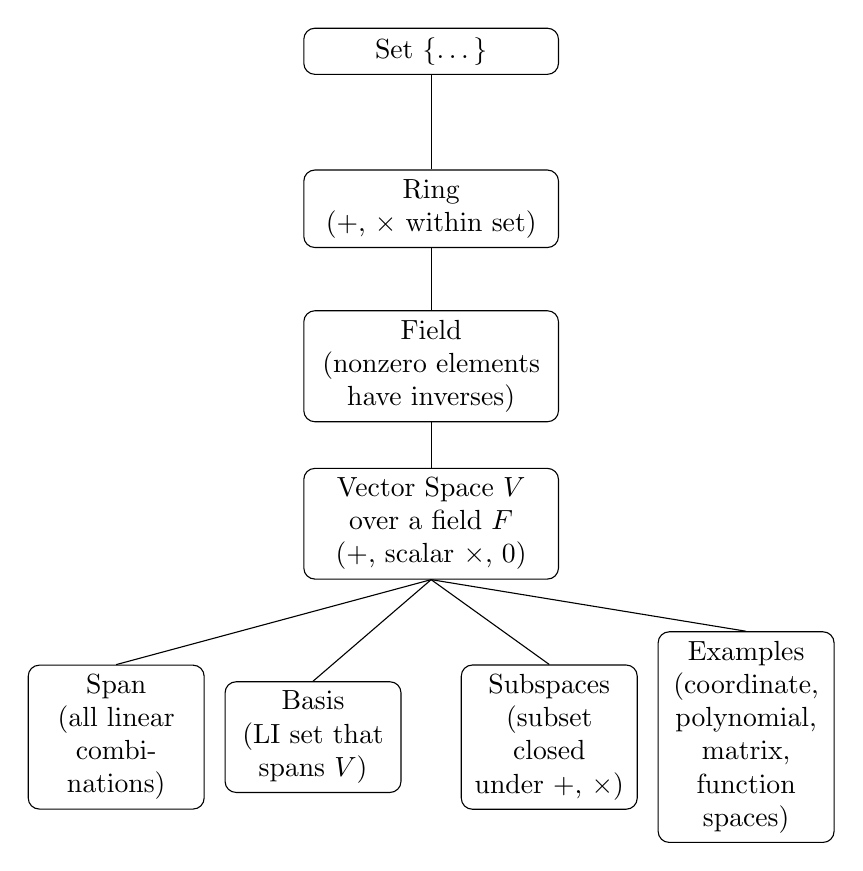
\begin{tikzpicture}[every node/.style={draw,rectangle,rounded corners,align=center, text width=3cm}, level distance=2cm, sibling distance=6cm]
        \node (set) {Set $\{ \dots \}$}
            child {node (ring) {Ring \\ (+, $\times$ within set)}
                child {node (field) {Field \\ (nonzero elements have inverses)}
                    child {node (VS) {Vector Space $V$ over a field $F$ \\ (+, scalar $\times$, 0)}} 
                }
            };
        \path (VS.south) ++(-4,-2) node[text width=2cm] (span) {Span \\ (all linear combinations)};
        \path (VS.south) ++(-1.5,-2) node[text width=2cm](basis) {Basis \\ (LI set that spans $V$)};
        \path (VS.south) ++(1.5,-2) node[text width=2cm](sub) {Subspaces \\ (subset closed under +, $\times$)};
        \path (VS.south) ++(4,-2) node[text width=2cm](examples) {Examples \\ (coordinate, polynomial, matrix, function spaces)};
        \draw (VS.south) -- (span.north);
        \draw (VS.south) -- (basis.north);
        \draw (VS.south) -- (sub.north);
        \draw (VS.south) -- (examples.north);
    \end{tikzpicture}
\end{center}

\noindent
This tree shows how vector spaces arise from fields (which arise from rings), and highlights the main concepts inside a vector space: spans, bases, subspaces, and common examples.

\paragraph{Rings vs Vector Spaces.} Although rings and vector spaces both have addition and a zero element, they differ fundamentally in how multiplication works:

\begin{itemize}
    \item \textbf{Ring:} A set $R$ with addition and multiplication between elements of $R$. Addition forms an abelian group, multiplication is associative, and distributes over addition. Scalars are elements \emph{inside the set}.
    \item \textbf{Vector Space:} A set $V$ with addition and multiplication by scalars from a \emph{field} $F$. Addition forms an abelian group, scalar multiplication distributes appropriately. There is no multiplication between vectors themselves; only scalar multiplication is defined.
\end{itemize}


\section{Solutions}
\begin{solution}[Invertibility]
    Suppose \(B\) and \(B'\) are both inverses of \(A\). Then
    \[B = B I = B(AB') = (BA)B' = I B' = B'.\]
    Therefore, \(B = B'\), so the inverse is unique.
\end{solution}
\begin{solution}[Invertibility 2]
    We can answer this problem with proof by contradiction. Let's
    suppose this matrix is invertible. By definition there exists B = $\begin{pmatrix}a&b\\c&d\end{pmatrix}$ such that $\begin{bmatrix}0&1\\0&0\end{bmatrix}$ $\begin{bmatrix}a&b\\c&d\end{bmatrix}$ = $\begin{bmatrix}1&0\\0&1\end{bmatrix}$.  We can rewrite this equation into: $\begin{bmatrix}a&b\\c&d\end{bmatrix}$ = $\begin{bmatrix}0&1\\0&0\end{bmatrix}^{-1}$. The inverse of our matrix can be rewritten as $\frac{1}{0*0 - 1*0}\begin{bmatrix}0&-1\\0&0\end{bmatrix}$\footnote{Recall that an inverse of a $2 \times 2$ matrix is equal to its determinant multiplied with its conjugate}. But this is undefined since division by 0 is undefined. Therefore, our initial assumption that the matrix is invertible is false, and thus the matrix is not invertible.
\end{solution}
\begin{solution}[Field]
    A field with 2 elements can be constructed as follows:
    Let \(F = \{0, 1\}\) be a set with two elements. We define addition and multiplication operations on \(F\) as follows:
    \begin{itemize}
        \item \(0 + 0 = 0\)
        \item \(0 + 1 = 1\)
        \item \(1 + 0 = 1\)
        \item \(1 + 1 = 0\)
        \item \(0 \times 0 = 0\)
        \item \(0 \times 1 = 0\)
        \item \(1 \times 0 = 0\)
        \item \(1 \times 1 = 1\)
    \end{itemize}
\end{solution}
\begin{solution}[Span]
    \[\Span(v_1,v_2) = \{xv_1 + yv_2 : x,y \in \mathbb{R}\} = \left\{\begin{pmatrix}3x + y\\x + 3y\end{pmatrix}: x,y \in \mathbb{R}\right\}.\]
\end{solution}
\begin{solution}[Span 2]
    Assume $u = a u_1 + b u_2 + c u_3$, with $a,b,c \in \mathbb{R}$. This gives the system of equations
    \[\begin{amatrix}{3}3 & 1 & 2 & 2 \\ 10 & 3 & 8 & 10 \\ 7 & -2 & 1 & 7\end{amatrix}.\]
    Solving via Gaussian elimination, we find $a = \frac{2}{21}$, $b = -\frac{46}{21}$, and $c = \frac{41}{21}$. Hence $u \in \Span(u_1,u_2,u_3)$.
\end{solution}
\begin{solution}[Subspace Criterion]
    Let $A \in M_n(K)$ be fixed and define
    \[U = \{x \in K^n : Ax = \vec{0}\}.\]
    We verify the subspace criterion.

    (0) Non-empty:  
    Since $A0 = 0$, we have $0 \in U$.

    (1) Closed under addition:  
    Let $x,y \in U$. Then $Ax = 0$ and $Ay = 0$. Hence
    \[A(x+y) = Ax + Ay = 0 + 0 = 0,\]
    so $x+y \in U$.

    (2) Closed under scalar multiplication:  
    Let $x \in U$ and $\lambda \in K$. Then
    \[A(\lambda x) = \lambda Ax = \lambda 0 = 0,\]
    so $\lambda x \in U$.

    Therefore, by the subspace criterion, $U$ is a subspace of $K^n$. It is called the null space (kernel) of $A$.
\end{solution}
\begin{solution}[Subspace Criterion 2]
    We verify the subspace criterion.

    (0) Non-empty:  
    Since $A0 = 0$, we have $0 \in U$.

    (1) Closed under addition:  
    Let $y_1,y_2 \in U$. Then there exist $x_1,x_2 \in K^n$ such that
    \[y_1 = Ax_1, \quad y_2 = Ax_2.\]
    Hence,
    \[y_1 + y_2 = Ax_1 + Ax_2 = A(x_1 + x_2) \in U.\]

    (2) Closed under scalar multiplication:  
    Let $y \in U$ and $\lambda \in K$. Then $y = Ax$ for some $x \in K^n$, and
    \[\lambda y = \lambda Ax = A(\lambda x) \in U.\]

    Therefore, by the subspace criterion, $U$ is a subspace of $K^n$. It is called the image of $A$.
\end{solution}
\begin{solution}[Subspace Criterion 3]
    Let $U \subseteq K$ be a subspace. We show that either $U = \{0\}$ or $U = K$. If $U = \{0\}$, we are done. Otherwise, $U \neq \{0\}$. Then there exists $v \in U$ with $v \neq 0$.
    We prove that $U = K$. Let $x \in K$ be arbitrary. Since $v \neq 0$, there exists $\lambda \in K$ such that
    \[x = \lambda v.\]
    Because $U$ is closed under scalar multiplication, $\lambda v \in U$, hence $x \in U$. Therefore every $x \in K$ belongs to $U$, so $U = K$. Conclusion: the only subspaces of $K$ are $\{0\}$ and $K$.
\end{solution}
\begin{solution}[Subspace Criterion 4]
    We verify the subspace criterion.
    (0) Non-empty:  
    Taking $\lambda_1=\cdots=\lambda_n=0$ gives
    \[0 = 0v_1 + \cdots + 0v_n \in \Span(v_1,\dots,v_n).\]
    (1) Closed under addition:  
    Let $u,v \in \Span(v_1,\dots,v_n)$. Then there exist scalars
    $a_1,\dots,a_n,b_1,\dots,b_n \in K$ such that
    \[u = a_1 v_1 + \cdots + a_n v_n, \quad v = b_1 v_1 + \cdots + b_n v_n.\]
    Hence,
    \[u+v = (a_1+b_1)v_1 + \cdots + (a_n+b_n)v_n \in \Span(v_1,\dots,v_n).\]
    (2) Closed under scalar multiplication:  
    Let $u \in \Span(v_1,\dots,v_n)$ and $\lambda \in K$. Then
    \[u = a_1 v_1 + \cdots + a_n v_n\]
    for some scalars $a_i$, and
    \[\lambda u = (\lambda a_1)v_1 + \cdots + (\lambda a_n)v_n \in \Span(v_1,\dots,v_n).\]
    Therefore, $\Span(v_1,\dots,v_n)$ is a subspace of $V$.
\end{solution}
\begin{solution}[Span Membership]
    We look for scalars $x,y,z \in \mathbb{R}$ such that
    \[xv_1 + yv_2 + zv_3 = v.\]
    That is,
    \[x\begin{pmatrix}1\\2\\1\end{pmatrix} + y\begin{pmatrix}2\\5\\4\end{pmatrix} + z\begin{pmatrix}1\\3\\6\end{pmatrix} = \begin{pmatrix}3\\5\\-5\end{pmatrix}.\]
    This gives the system
    \[\begin{cases}
    x + 2y + z = 3,\\
    2x + 5y + 3z = 5,\\
    x + 4y + 6z = -5.
    \end{cases}\]
    Solving, we obtain
    \[x=3,\quad y=1,\quad z=-2.\]
    Therefore,
    \[v = 3v_1 + v_2 - 2v_3,\]
    so $v \in \Span(v_1,v_2,v_3)$.
\end{solution}
\begin{solution}[Span Membership 2]
    We seek scalars $x,y,z \in \mathbb{R}$ such that
    \[f = xf_1 + yf_2 + zf_3.\]
    Comparing coefficients,
    \[x(x^2+2x+1) + y(2x^2+5x+4) + z(x^2+3x+6) = 3x^2+5x-5,\]
    which gives
    \[\begin{cases}
    x + 2y + z = 3,\\
    2x + 5y + 3z = 5,\\
    x + 4y + 6z = -5.
    \end{cases}\]
    Solving,
    \[x=3,\quad y=1,\quad z=-2.\]
    Hence,
    \[f = 3f_1 + f_2 - 2f_3,\]
    and therefore $f \in \Span(f_1,f_2,f_3)$.
\end{solution}

\section{Useful Links}

\end{document}